\documentclass[12pt]{report}

\usepackage{setspace}
\usepackage{fancyhdr}
\usepackage{psfrag,amsmath,amsthm,graphicx,subfigure}
%\usepackage[round]{natbib}
\usepackage{vmargin}

\usepackage{graphicx}
\usepackage{algorithm}
\usepackage{algorithmic}
\usepackage{amsfonts}
\usepackage{verbatim}
\usepackage{subfigure}

\setpapersize{A4}
\setmarginsrb{3.6cm}{1.95cm}{2.5cm}{1.95cm}{1cm}{1cm}{1cm}{2cm}
\renewcommand{\headrulewidth}{0.2pt}

\newenvironment{romanpages}{\cleardoublepage\setcounter{page}{1}\renewcommand{\thepage}{\roman{page}}}

{\cleardoublepage\renewcommand{\thepage}{\arabic{page}}\setcounter{page}{1}}

%\graphicspath{{Figures/}}


%\newtheorem{theorem}{Theorem}[section]
%\newtheorem{lemma}[theorem]{Lemma}
%\newtheorem{proposition}[theorem]{Proposition}
%\newtheorem{corollary}[theorem]{Corollary}



%\newtheorem{theorem}{Theorem}[section]
%\newtheorem{Note}{Note}[section]
%\newtheorem{Corollary}{Corollary}[section]

\newcommand{\Xb}{\ensuremath{\mathbf{X}}}

% __________________________________________________________________

\begin{document}

\begin{titlepage}

\LARGE \centerline{\bf Fast Growing and Interpretable Oblique Trees \rm }
\LARGE \centerline{\bf via Logistic Regression Models \rm }
\vspace{3em}
\large \centerline{Alfred Truong}
\vspace{0.5em}
\large \centerline{Christ Church College}
\vspace{0.5em}
\large \centerline{University of Oxford}
\vspace{2em}
\begin{figure} [h!]
\begin{center}

\includegraphics[width=0.5\textwidth]{Oxlogo_BW_lg.eps}
\end{center}
\end{figure}
\vspace{2em}
\large \centerline{\emph{A Thesis submitted for the degree of Doctor of Philosophy}}
\vspace{3em}
\large \centerline{Hilary Term 2009}

\end{titlepage}

\pagebreak
\thispagestyle{empty}

\vspace*{17cm}

Acknowledgements

\pagebreak
\thispagestyle{empty}

\begin{center}
\large \bf Fast Growing and Interpretable Oblique Trees via Logistic Regression Models
\end{center}
\vspace*{0.5cm}
\centerline{\bf Alfred Truong, Christ Church College}
\vspace*{0.5cm}
\centerline{\bf DPhil thesis, Department of Statistics}
\vspace*{0.5cm}
\centerline{\bf Hilary Term 2009}
\vspace*{0.5cm}

The key strength of classification trees is its interpretability which unfortunately diminishes as a tree gets larger. The reason for this is the interplay between the distribution of class observations and the splits that are used to partition them. Widely used methods of tree growth apply axis-parallel splits on continuous attributes ($X_i<c$) even though oblique splits ($\sum_i a_iX_i<c$) are better suited for the task. Though many have found ways to grow oblique trees, existing methods have not caught on. This thesis identifies possible reasons for this and seeks to address them by proposing a new approach to growing oblique trees. An intuitively appealing approach is suggested that is easily extensible which allows more interpretable oblique trees to be found. 

\pagebreak
\thispagestyle{empty}
\vspace*{7cm}
\section*{Declaration}
I declare that this thesis is wholly my own work unless otherwise stated. No part of this thesis has been accepted or is currently being submitted for any degree or diploma or certificate or other qualification in this university or elsewhere.\\\\
Candidate: Alfred TRUONG\\\\
Signed:\\\\
Date:\\\\

%\pagebreak

\begin{romanpages}
\doublespacing
\tableofcontents
%\listoffigures
%\listoftables
\end{romanpages}	
% __________________________________________________________________________

\fancyhead[RO,LE]{\thepage}
\fancyhead[LO]{\nouppercase{\rightmark}}
\fancyhead[RE]{\nouppercase{\leftmark}}
\pagestyle{fancy}

\doublespacing
\chapter{Introduction}
\label{Introduction}

\section{Recent Trends in Statistics}
\label{RecentTrendsinStatistics}
Data-storage and data-capture devices have consistently become both cheaper and more powerful allowing enormous amounts of data to be collected. The computational power of computers needed to sift through this data has also increased exponentially\footnote{Increases in computational power have so far grown according to Moore's Law (1965)~\cite{Moore1965} which roughly states that the number of transistors in integrated circuits doubles every 2 years.}. With enormous pools of specialist commercial and scientific data that have since been amassed, there is great potential for knowledge discovery from these databases. Prime examples include data gathered from supermarket loyalty cards, the Human Genome Project and the Internet. The ability to understanding consumer shopping habits, predispositions to genetic disorders and helping people find information on the Internet holds great commercial value.\\

Applied Statisticians have made great strides in this area tackling data-related problems ranging from Bioinformatics to Optical Character Recognition and have done so by marrying the power of computers with ideas from Statistics. In doing so, they have greatly increased the range of problems that Statistics can be used to tackle. \\

Though much progress has been made in the field of Pattern Recognition, it is often difficult for non-specialist users to apply such techniques to real-world datasets as academic work is often too specialized for easy use and proprietary software often written for profit. As a result, such ideas cannot have reached their full potential. There has however been movement in recent years towards providing widely accessible open-source software\footnote{R~\cite{R} is a free software environment for statistical computing which gathers open-source implementations of an extensive collection of statistical and graphical techniques. It has become a defacto standard for developers of statistical software due to its highly extensible nature and its ease of use.} to address these issues via a program called R. With vast improvements in computational power and a growing collection of easily extensible statistical programs, it has become worthwhile to revisit problems that were once considered too difficult. 

%The computational power of computers has increased by an order of a thousand since the early 1980's till now
\section{Aim of this Thesis}
\label{AimofthisThesis}
The Classification Tree is a widely used classifier introduced in its current form by Breiman \emph{et al}~\cite{cart84-2} in the 1980's. Like all other classifiers, a Classification Tree is simply a model that makes predictions of the class of previously unobserved observations as illustrated in Figure~\ref{fig_typical_classifier}. \\
\begin{figure}
\centering
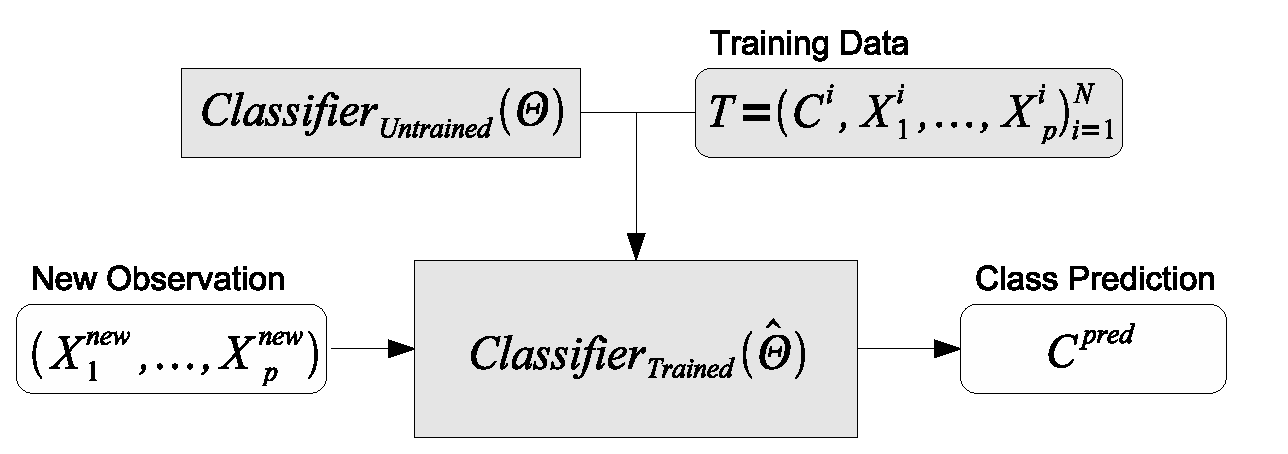
\includegraphics[width=1\textwidth]{fig_typical_classifier.eps}
\caption{A classification model makes predictions of the class of observations by viewing attributes $\left(X_1^{new},\ldots,X_p^{new}\right)$ measured from it. A classifier must firstly be trained to some data $\mathcal{T}$ to find parameters that allow it to model observations from such a population. A trained classifier can therefore make informed predictions of the class $C^{pred}$ of previously unobserved observations.}
\label{fig_typical_classifier}
\end{figure}

The main strength of a Classification Tree is the simplicity with which it makes these predictions. One follows a flow diagram (called a tree) performing a series of predefined tests which eventually leads to a prediction. It is an interpretable and opaque process which appeals to many practitioners.\\

Though there are many possible applications of this idea, Classification and Regression Trees (CART trees) proposed by Breiman \emph{et al} are the most widely used form. It mainly focuses on using dichotomous tests of the form $X_i<c$ (axis-parallel splits) over continuous attributes for two main reasons, 
\begin{itemize}
\item[-] axis-parallel splits are interpretable and 
\item[-] more importantly they are easy to implement even for large datasets.
\end{itemize}
Though CART trees are considered to be interpretable relative to other classifiers, its interpretability diminishes with the size of a tree (the number of tests it uses) so it is desirable to find ways of obtaining smaller trees. One way of achieving this is to consider more general tests, say of the form $\sum_i a_iX_i<c$ (summing over continuous attributes $X_i$). Such tests will be called oblique splits\footnote{Tests of the form $\sum_i a_iX_i<c$ have been known by many names as many researchers have worked on incorporating them into trees. Other names include Linear Machines, Linear-Combination Tests, Multivariate Tests and Oblique Splits.}.\\

Though many attempts have been made at growing\footnote{Trees are said to be grown as well as trained to training data.} oblique trees (trees grown by considering oblique splits over continuous attributes), none have caught on; axis-parallel trees (those that consider axis-parallel splits over continuous attributes) are still widely used. This thesis aims to identify and address potential reasons for this so that oblique trees may be better utilized.

\section{Organization of this Thesis}
\label{OrganizationofthisThesis}
This thesis is organized as follows. Chapter~\ref{Introduction} contains a brief overview of recent developments in Information Technology and its relation to modern Applied Statistics. A description of the aim of this thesis follows with an overview of the thesis. \\

Chapter~\ref{Background} identifies possible reasons as to why existing approaches to growing oblique trees are shunned. Starting with a recap of the basic idea of a Classification Tree, a discussion on how oblique splits might be used to improve tree interpretability is given. A summary of likely reasons for their lack of use follows. \\

Chapter~\ref{ExistingWork} surveys existing approaches to growing oblique trees. Existing work is separated into the two philosophies by which they find oblique splits to provide a clearer understanding of the material as well as its progression. \\

Chapter~\ref{ObliqueSplitsviaProbabilisticModels} presents a new approach to finding oblique splits with real-life examples. A heuristic argument further backing the proposed approach is follows. \\

!!!!!!!!!!!!!!!!!!!!!
Chapter~\ref{InterpretableObliqueTrees} present methods of obtaining interpretable oblique trees. Methods are broadly separated into two groups, those applied during tree growth and those applied post-tree growth.\\

An in-depth analysis of techniques presented in this thesis are given in Chapter~\ref{AdditionalPoints}. It explores its weaknesses and limitations and highlights situations where it performs well.\\

Chapter~\ref{ConcludingRemarks} concludes with final remarks for work in this thesis.
\chapter{Background}
\label{Background}
This chapter presents the basic idea of a Classification Tree and reviews issues involved when training CART trees to data. By covering various aspects of tree growth, likely reasons as to why existing approaches to growing oblique trees have not caught on are identified. Section~\ref{ClassificationTrees} revisits the idea of a Classification Tree and Section~\ref{TreeInterpretability} follows with a discussion of issues that affect the interpretability of a tree. Doing so demonstrates why oblique splits are sometimes be better suited for growing interpretable trees. Unfortunately, oblique splits are inherently difficult to use as will be explained in Section~\ref{FindingObliqueSplits}. A list of possible explanations why existing approaches to growing oblique trees have not caught on follow in Section~\ref{PossibleReasonsforStatusQuo}.

\section{Classification Trees}
\label{ClassificationTrees}
\subsection{Natural Origins}
\label{NaturalOrigins}
The idea of tree-based classification appears naturally when considering populations with hierarchical structure and is nothing new. Biologists have long used this idea to help identify organisms, botanists to name plants~\cite{nla.cat-vn178734}~\cite{nla.cat-vn2380672} and doctors to assist medical diagnoses~\cite{609112}~\cite{AnneB.Nattinger04011998}. Tree-based classifiers allow subject specialists to distill expert knowledge into a set of easily understandable and transparent rules for others to follow. Figure~\ref{fig_taxonomy_key_biology_table} shows a simple application of this idea in Biology.
\begin{figure}
\centering
\subfigure[Taxonomic Key for various species of plants.]{
    \label{fig_taxonomy_key_biology_table}
	\includegraphics[width=.47\textwidth]{fig_taxonomy_key_biology_table.eps}
}
\subfigure[Graphical representation of information contained in Taxonomic Key.]{
    \label{fig_taxonomy_key_biology_tree}
	\includegraphics[width=.47\textwidth]{fig_taxonomy_key_biology_tree.ps}
}
\caption{Tree-based classification is a natural way of classifying hierarchical populations and has long been used by practitioners from various fields. A Dichotomous Taxonomic Keys in particular ask a series of questions with \emph{Yes} or \emph{No} answers as shown in Figure~\ref{fig_taxonomy_key_biology_table}. It is easy to follow and each path leads to a class prediction. This information can also be represented by a tree (where left branches by convention denote positive answers).}
\label{fig_taxonomy_key_biology}
\end{figure}
Armed with this Taxonomic Key, anyone can easily identify species of plants specified in the Key. If a plant has shoots and does not flower, it is a Pine Tree. If it shoots and flowers but does not have leaves, it is a Cactus Tree. The information contained in this construct can also be shown graphically by a tree as seen in Figure~\ref{fig_taxonomy_key_biology_tree}.\\

Though a great deal of thought is often needed to create such Taxonomic Keys manually, researchers have sought ways of automating this process to extract information from databases in general. The question they have in mind is as follows,
\begin{quote}
\emph{Can tree-based classifiers be automatically grown to data in such a way that they can be used to accurately predict the class of previously unobserved observations?}
\end{quote}
Working independently, researchers from Computer Science~\cite{Quinlan.86}~\cite{Quinlan.88}~\cite{Quinlan.90} and Applied Statistics~\cite{cart84-2} arrived at similar solutions to this problem. With greater cross-fertilization of ideas and additional input from the Engineering community~\cite{Sethi.Sarvarayudu.82}, Breiman \emph{et al} proposed the widely accepted \emph{Classification and Regression Trees} algorithm in 1984 still widely used today. An overview of these ideas follow.

\subsection{Tree Growth}
\label{TreeGrowth}
Given classification data of the form $\mathcal{T}=\left(C^i,X_1^i,\ldots,X_p^i\right)_{i=1}^N=\left(C^i,\Xb^i\right)_{i=1}^N$, a Classification Tree is grown to it by recursively partitioning observations into smaller subsets where observations have more similar classes. This process is naturally representable as a tree with
\begin{itemize}
\item[-] internal nodes were tests partition observations,
\item[-] branches from nodes which represent the outcomes of these tests and
\item[-] leaves at the bottom\footnote{Trees are conventionally drawn with its root at the top of a page growing downwards.} of the tree.
\end{itemize}
When using Classification Trees for prediction, observations are passed through the tree and classified by the class associated to the leaf where it falls. These ideas are illustrated in Figure~\ref{fig_typical_CART_tree}.
\begin{figure}
\centering
\subfigure[Example of a binary splitting axis-parallel tree.]{
	\label{fig_typical_CART_tree_plot_tree}
	\includegraphics[width=.47\textwidth]{fig_typical_CART_tree_plot_tree.ps}
}
\subfigure[The associated decision boundaries defined by the tree on the feature space.]{
	\label{fig_typical_CART_tree_decision_boundaries}
	\includegraphics[width=.47\textwidth]{fig_typical_CART_tree_decision_boundaries.ps}
}
\caption{The above tree is grown to a training set where observations have two continuous attributes $p=2$ with observations from four classes $C\in\left\{1,\ldots,4\right\}$. Four dichotomous tests are applied at internal nodes to produce five leaves. The classes associated to each leaf are shown at the bottom of a tree. With $p=2$, it is possible to view the associated decision boundaries defined by the tree on the feature space $\Xb=\mathbb{R}^2$. As axis-parallel splits are used to partition observations, the feature space is partitioned with rectangular blocks.}
\label{fig_typical_CART_tree}
\end{figure}
As can be seen, five tests partition observations from four classes and good separation is achieved between observations of each class.\\

Though the idea of a Classification Tree allows arbitrarily complex tests at internal nodes, CART trees focus on univariate binary splits to simplify the problem. Tests are univariate in that only one attribute is used to construct each test and binary in that they result in exactly two outcomes. Trees grown in this manner partition observations into (high-dimensional) rectangular blocks as seen in Figure~\ref{fig_typical_CART_tree_decision_boundaries}.\\

With $p$ attributes in total (of which $q$ are continuous say), many tests can be applied during tree growth at each internal node. The exact form of tests considered by CART trees depends on the type of data it is based on.
\begin{description}
\item[$X_i$ continuous:] tests are constrained to be of the form $X_i<c$ v.s. $X_i\geq c$ for some constant $c\in\mathbb{R}$
\item[$X_i$ categorical:] tests are constrained to be of the form $X_i\in A$ v.s. $X_i\notin A$ for some subset $A$ of the factors of the categorical attribute $\left\{a_1,\ldots,a_{|X_i|}\right\}$ 
\end{description}
Of the numerous tests that exist, the one ``best partitioning observations of each class'' (the best split) is applied and the process repeated on child nodes. An impurity measure to compare tests (somehow quantifying this concept) is used. This is examined in greater detail later on.\\

Having understood the generative process of recursive partitioning, we consider two techniques employed by CART trees to avoid overfitting\footnote{Highly parameterized statistical models can fit training data perfectly (low variance) though will not predict well to previously unobserved observations (high bias); the bias-variance tradeoff~\cite{Geu02}~\cite{citeulike:161814}.}. The first employs the early stopping of recursive partitioning during tree growth and the logic is simple, 
\begin{itemize}
\item[-] if recursive partitioning proceeds until all training set observations are perfectly classified, the tree is like to have focused more on specific occurrences in the training set rather than generalities in the population,
\item[-] recursive partitioning should therefore stop before leaves become pure (observations at each leaf are all of the same class)
\end{itemize}
To achieve this, recursive partitioning terminates at a node if any of the following criteria are satisfied,
\begin{description}
\item[Pure Nodes:] if all observations at a node are of the same class, recursive partitioning terminates (further partitions add no value).
\item[Size Threshold:] if a node contains fewer than some prespecified number of observations (defaulted to 10), recursive partitioning terminates (trees should not focus on small details). 
\item[Impurity Threshold:] if impurity at a node is below some prespecified proportion of that of the entire training set (defaulted to 0.01), recursive partitioning terminates (such nodes are considered to be \emph{sufficiently pure}).
\item[Child Node Threshold:] if applying the best split produces a child node with fewer than some prespecified number of observations (defaulted to 5), recursive partitioning terminates (leaves should not become too specialized).
\end{description}
Unfortunately, early stopping is not sufficient to ensure that resulting CART trees generalize\footnote{A classifier that generalizes is one that is not overfit; it makes good class predictions for previously unobserved observations.}. Breiman \emph{et al} propose the following complementary technique to address this issue.

\subsection{Cost-Complexity Pruning}
\label{CostComplexityPruning}
Growing trees that generalize can be thought of as tackling an optimal stopping problem for the recursive partitioning process (trees should be grown to data to learn from it but they should not be overgrown). When exactly should one stop? \\
%This allows all avenues to be investigation during tree growth and allows a simple generalizing tree to be obtained. \\
%Early stopping prevents trees from focusing on small details, it can also obstructing the discovery of potentially useful splits (recursive partitioning may terminate just as tree growth is onto something).

Cost-complexity pruning avoids this question altogether by simply growing a tree until it is overfit (a maximal tree) and by ``looking backwards from it'' to find rooted subtrees of it that \emph{do} generalize. Instead of considering all possible rooted subtrees\footnote{The number of rooted subtrees of a maximal tree is potentially vast. For binary trees with $l$ leaves, Breiman \emph{et al}~\cite{cart84-2} pg. 284 calculate an upper bound to be $\lfloor 1.5028369^l\rfloor$ with an exact bound in the case of saturated trees (trees with $n$ levels of internal nodes with a full complement of $2^n$ leaves). A 3-levelled saturated tree has $26 = \lfloor (1.5028369)^{2^3}\rfloor$ rooted subtrees while a 4-levelled saturated tree has $677 = \lfloor (1.5028369)^{2^4}\rfloor$. All rooted subtrees of a 3-levelled saturated tree are identified in Figure~\ref{fig_rooted_subtrees}. It is easy to see the multiplicative effect that each internal node has on the total number of rooted subtrees.}\begin{figure}
\centering
\includegraphics[width=1\textwidth]{fig_rooted_subtrees.ps}
\caption{A 3-levelled saturated tree is shown in the top-left plot with its nodes labeled. The other plots show its rooted subtrees, rows 1 to 4 showing those where neither nodes 2 and 3 are absent, row 5 showing those where only node 3 is absent, row 6 showing those where only node 2 is absent and the rest follow on the last row. One sees that the total number of rooted subtrees grows in a multiplicative manner with each additional internal node.}
\label{fig_rooted_subtrees}
\end{figure}, cost-complexity pruning focuses on a specific subset of them found as follows. For trees $T$, let
\begin{description}
\item[$R(T)$] denote a measure of its goodness of fit found by adding contributions $r(t)$ over its leaves $t$ (the number of misclassifications or impurity say) and
\item[$size(T)$] denote a penalty measure that increases as trees become ``more complex'' (the number of leaves say)
\end{description} 
then use the following measure to compare rooted subtrees of a maximal tree $$R_k(T)=R(T)+k~size(T).$$
For any given $k$, $R_k(T)$ weights the ability of a rooted subtree $T$ to fit training data against its complexity allowing comparison of rooted subtrees. Breiman \emph{et al} propose focusing on rooted subtrees that minimize $R_k(T)$ for each value of $k\in\mathbb{R}$. Amazingly, Breiman \emph{et al} show\footnote{Concise version of these proofs are found in Ripley~\cite{Ripley.96}.}~\cite{cart84-2} pg. 284--293 that a nested family of rooted subtrees $\left\{T_i\right\}_{i=0}^K$ is optimal over all $k$ and that each $T_i$ is optimal over some range $k\in[k_i,k_{i+1})$ with $$-\infty=k_0<k_1<\ldots<\infty.$$ In addition to this, they also give a method for finding the $k_i$'s as well as an algorithm to construct the entire tree sequence $\left\{T_i\right\}_{i=0}^K$. The cost-complexity tree that best generalizes is easily identified and used as the final classifier. The entire process is a illustrated in Figure~\ref{fig_tree_pruning}. 
\begin{figure}
\centering
\includegraphics[width=1\textwidth]{fig_tree_pruning.ps}
\caption{Cost-complexity pruning allows trees that generalize well to be found. Starting with a fully grown (and thus overfit tree), a family of rooted subtrees $\left\{T_i\right\}_{i=0}^K$ is easily extracted from it to be used as candidates for the final classifier. Trees in $\left\{T_i\right\}_{i=0}^K$ are nested with increasing $i$ and each $T_i$ minimizes $R_k(T)$ over the range $k\in[k_i,k_{i+1})$. Though prediction error over the training set (in-sample error) increases with $i$, out-of-sample error needed not; the best generalizing tree is used as the final classifier. In the above example, $T_1$ say, might have the lowest out-of-sample prediction error and thus be used as the final classifier.}
\label{fig_tree_pruning}
\end{figure}

\section{Tree Interpretability}
\label{TreeInterpretability}
As mentioned previously, the interpretability of a tree is its main strength. Though each univariate binary split is interpretable in isolation, the interpretability of an entire axis-parallel tree need not be. Tree interpretability deteriorates as trees become larger as seen in Figure~\ref{fig_tree_interpretability}.\\
\begin{figure}
\centering
\includegraphics[width=.49\textwidth]{fig_tree_interpretability_more.ps}
\includegraphics[width=.49\textwidth]{fig_tree_interpretability_less.ps}
\caption{The interpretability of a tree depends on two factors, the interpretability of each split in isolation and its cumulative effect over the entire tree. A balance should be achieved between using simple tests that are easy to understand and more complex tests that allow smaller trees to be grown.}
\label{fig_tree_interpretability}
\end{figure}

The reason why some trees are larger than others simply comes down to the interplay between how observations of different classes are distributed over the feature space and the tests used to partition them; recursive partitioning will proceed until all leaves are sufficiently pure with whatever tests it is allowed to use. One way of obtaining smaller trees is to consider more general splits during tree growth. For tests over continuous attributes, a multivariate generalization of axis-parallel splits is an oblique split $\sum_{i=1}^q a_iX_i<c$ (assuming continuous attributes lie in the first $q$ positions). Oblique splits are better suited to partitioning observations as shown in Figure~\ref{fig_power_of_splits}.\\
\begin{figure}
\centering
\subfigure[A single oblique split is enough to partition observations in this example.]{
	\label{fig_power_of_splits_oblique}
	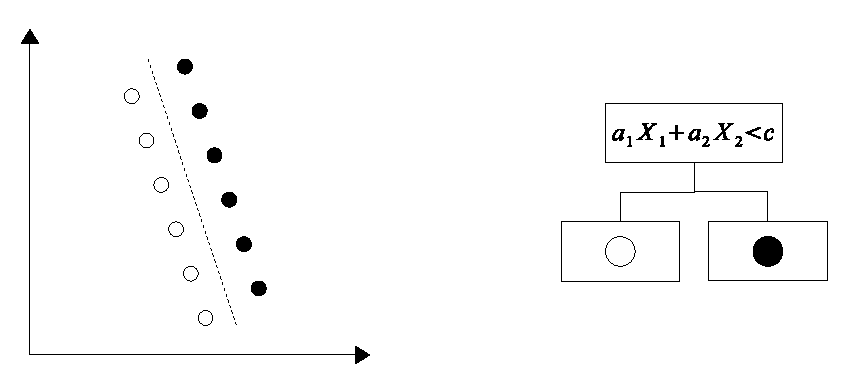
\includegraphics[height=4cm]{fig_power_of_splits_oblique.ps}
}
\subfigure[An axis-parallel tree requires more that one level of splits to achieve the same purity within its leaves as a single oblique split.]{
	\label{fig_power_of_splits_axis_parallel}
	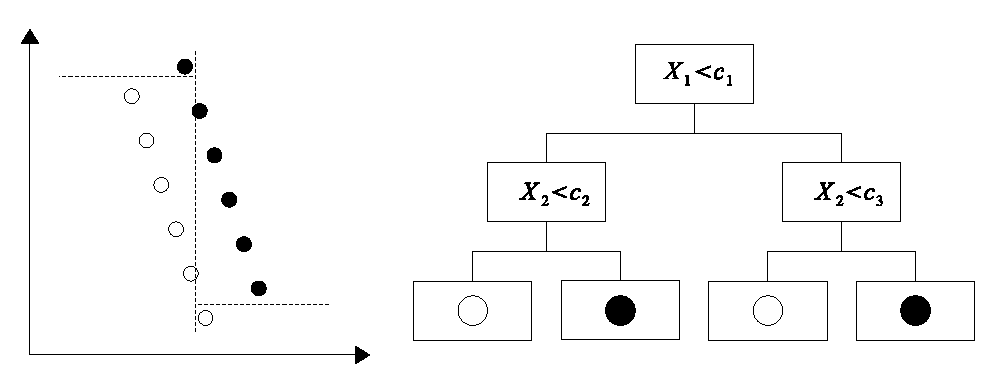
\includegraphics[height=4cm]{fig_power_of_splits_axis_parallel.ps}
}
\caption{Observations from this two-class classification problem are easily partitioned with a single oblique split as shown in Figure~\ref{fig_power_of_splits_oblique}. A single axis-parallel split however cannot produce the same partitioning requiring another level of splits to achieve the same result as shown in Figure~\ref{fig_power_of_splits_axis_parallel}. Oblique splits are better able at partitioning observations so oblique trees should be smaller than axis-parallel trees.}
\label{fig_power_of_splits}
\end{figure}

Though oblique splits naturally result in smaller trees, they are not necessarily more interpretable. In calling oblique splits that use all $q$ continuous attributes full oblique splits, we state the obvious in that full oblique splits are less interpretable than those using fewer attributes, e.g. $X_1>0.25 X_2$ v.s. $X_1>0.25 X_2+0.5 X_3+X_4$. Unwarranted use of full oblique splits to grow oblique trees can paradoxically reduce interpretability as it results in ``cluttered trees'' (the problem becomes more acute with increasing $q$). Though oblique splits may be useful at time, concise oblique splits should always be used \emph{whenever possible} to obtain more interpretable trees.

\section{Finding Oblique Splits}
\label{FindingObliqueSplits}
Putting aside the issue of how one obtains interpretable oblique trees for the meantime, it is instructive to analyze the problem of finding the best full oblique split at each stage of tree growth. One ideally applies the test with the lowest impurity which implies that \emph{all oblique splits} must be considered. By introducing the idea of a split dictionary, it is possible to directly compare the magnitude of the computational problems posed when finding the best oblique split with that of the best axis-parallel split. \\

A split dictionary (for a family of splits) is a set of splits of minimal size that produces all possible partitioning of observations (permitted by that family of splits) over the training set. Figure~\ref{fig_split_dictionaries} shows possible axis-parallel and oblique split dictionaries for a small dataset.
\begin{figure}
\centering
\subfigure[Example of an axis-parallel split dictionary.]{
	\label{fig_split_dictionary_axis_parallel}
	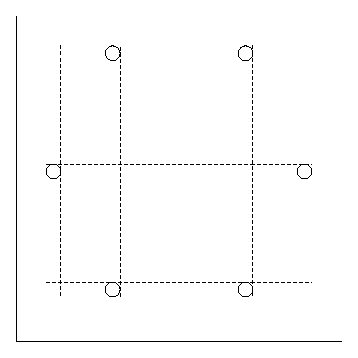
\includegraphics[width=.45\textwidth]{fig_split_dictionary_axis_parallel.eps}
}
\subfigure[Example of an oblique split dictionary.]{
	\label{fig_split_dictionary_oblique}
	
\includegraphics[width=.45\textwidth]{fig_split_dictionary_oblique.eps}
}
\caption{
A split dictionary (for a family of splits) is a set of splits of minimal size that produces all possible partitioning of observations (permitted by that family of splits) over the training set. Though split dictionaries need not be unique (small perturbations produce new split dictionaries), its size stays constant for a given dataset. Figure~\ref{fig_split_dictionary_axis_parallel} shows a possible axis-parallel split dictionary for a small dataset and is of size 6. No other partitioning of observations can result with axis-parallel splits other than those generated here. Figure~\ref{fig_split_dictionary_oblique} shows a possible oblique split dictionary for the same data and is of size 15 (it is larger as oblique splits can produce different partitions of the observations).}
\label{fig_split_dictionaries}
\end{figure}
Though there are often many split dictionaries for a family of splits, its size remains constant for a given dataset.\\

We start by considering axis-parallel splits $X_i<c$. For a generic training set $\mathcal{T}$ with $q$ continuous attributes of size $N$, though there may be uncountably many splits ($c\subset B\subseteq\mathbb{R}$), only a finite number of outcomes will ever occur over the training set. If there are $L_i$ unique values of $X_i$ in $\mathcal{T}$, there will therefore be exactly $L_i-1$ unique outcomes over attribute $X_i$. The size of the axis-parallel split dictionary (for all attributes) is therefore $\sum_{i=1}^q (L_i-1)$. With each $L_i$ at most $N$, the axis-parallel split dictionary can be seen to grow at most linearly in both $N$ and $q$.\\

A direct calculation of the size of the oblique split dictionary is very difficult. Fortunately however its size can be shown to be exactly $\left\{2\sum_{k=0}^{q} {L_{gen}-1\choose k}-2\right\}/2$ where $L_{gen}$ is the number of generally positioned\footnote{A set of $q$-dimensional vectors are generally positioned if every subset of size $q$ or less is linearly independent.} $q$-dimensional points in $\mathcal{T}$ and is a consequence of a combinatorial geometry result\footnote{Given $L_{gen}$ generally positioned points in $q$-dimensional space, there are exactly $2\sum_{k=0}^{q-1} {L_{gen}-1\choose k}$ ways of partitioning them into two bins as specified by which side of the hyperplane $\left\{x:w\cdot x=0\right\}$ they fall. Cover (1965) extended this result to enumerate the number of ways there are to partition points with more general hyperplanes of the form $\left\{x:w\cdot \phi(x)=0\right\}$ for general functions $\phi()$. Choosing $\phi(x)=(1,x)$ in particular shows there are exactly $2\sum_{k=0}^{q} {L_{gen}-1\choose k}$ ways of binning points across hyperplanes with arbitrary intercept. This includes the trivial cases where all points are assigned to the same bin and also double counting across bins.} by Cover~\cite{Cover65}. Assuming $L_{gen}$ is similar to $N$ (it can only be much less if all $q$-dimensional observations from the training set lie in a space of much lower dimensionality) shows that the oblique split dictionary grows extremely fast in both $N$ and $q$. \\

As $N$ and $q$ are often large in real-life datasets, it is practically impossible to find the best oblique split at each stage of tree growth. Existing approaches to growing oblique trees avoid this computational explosion in one of two ways,
\begin{itemize}
\item[-] choosing to focus on a subset of the oblique split dictionary
\item[-] searching for the best split while enforcing an early stop
\end{itemize}
A suboptimal oblique split is and can only be used. Further details follow in Chapter~\ref{ExistingWork}.

\section{Possible Reasons for Status Quo}
\label{PossibleReasonsforStatusQuo}
Though much work has been done on growing oblique trees, none of the existing approaches have caught on. Possible reasons as to why this might be are given below.
\begin{description} 
\item[Intellectual Appeal of the Approach:] Existing approaches to growing oblique trees find oblique splits in archaic ways. This does not give confidence to users in the suitability of such approaches. 
\item[Multiplicity of Trees:] To avoid the computational explosion noted in Section~\ref{FindingObliqueSplits}, some approaches find oblique splits stochastically which produces different a tree each time it is run. Though this is not necessarily a problem, no well-defined approach is given as to how one obtains a ``final classifier'' to use from many that can be grown. 
\item[Interpretability of Trees:] Most work is content with simply growing oblique trees with full oblique splits. Full oblique trees are not necessarily interpretable and so have no comparative advantage over other classifiers.
\item[Easily Accessible Implementations:] It is difficult to obtain and apply implementations of these approaches to real data.
\end{description}
%As has been shown in this chapter, it can be difficult to find oblique splits let alone growing an interpretable oblique tree. 
This thesis seeks to address each of these shortcomings by proposing an intellectually appealing approach to growing more interpretable oblique trees while providing an easily accessible implementation of this approach for others to use.
\chapter{Existing Work}
\label{ExistingWork} 
This chapter reviews existing approaches to growing oblique trees. As explained in Section~\ref{FindingObliqueSplits}, it is practically impossible to find the best oblique split during tree growth for all but the smallest of classification problems. Existing approaches avoid this in one of two ways.
\begin{description}
\item[Direct Search Approaches:] search for the split with the lowest impurity over the entire oblique split dictionary subject to some early stopping criteria.
\item[Indirect Search Approaches:] search for the split with the lowest impurity over some prespecified subset of the split dictionary.
\end{description}
Each approach has both strengths and weaknesses.\\

This chapter is organized as follows. Existing research is categorized into the above two categories and presented chronologically which provides a clear overview of its progression. Section~\ref{DirectSearchApproaches} presents direct search approaches and Section~\ref{IndirectSearchApproaches} follows with indirect search approaches. Section~\ref{SummaryofExistingWork} concludes this chapter by highlighting the inherent strengths and weaknesses of each approach.

\section{Direct Search Approaches}
\label{DirectSearchApproaches}
The approach taken by researchers for finding full obliques here can be summarized as follows, 
\begin{itemize}
\item[-] full oblique splits are essentially $q$-dimensional hyperplanes $\sum_{i=1}^q a_iX_i=c$
\item[-] hyperplanes can be thought of in terms of the vector $\left(a_i,\ldots,a_q,c\right)$ which in turn spans $\mathbb{R}^{q+1}$ 
%(vectors of coefficients are used to denote hyperplanes)
\item[-] defining a goodness/badness function $I()$ (over the training data) for hyperplanes, the best oblique split is simply the global maxima/minima over $\mathbb{R}^{q+1}$
\item[-] hill-climbing ideas can be applied to stochastically find good local maxima/minima under some early stopping regime
\end{itemize}
Though the computational problem of finding the best oblique split is still present, enforcing early stopping coupled with stochastic searches for local maxima/minima allows candidate splits to be found quickly. Though there is no guarantee such a maxima/minima found is the global extrema, a good solution suffices. A description of notable attempts follows.

\subsection{CART with Linear Combinations}
\label{CARTwithLinearCombinations}
Breiman \emph{et al} proposed one of the earliest direct search approaches as an aside in their CART book~\cite{cart84-2} (axis-parallel trees were the main focus of their work). Though they did not name their approach it has come to be known as ``CART with Linear Combinations'' (CART-LC) in the literature. \\

Their approach for finding oblique splits is as follows. Starting from the best axis-parallel split, look for a full oblique split that has a high value of $I()$ ``in close vicinity'' to this axis-parallel split by making small perturbations to it. Having found a suitable full oblique split, ``insignificant attributes'' are removed to reveal a more interpretable oblique split. A pseudocode description of this approach follows. \\

\begin{algorithm}
\caption{CART-LC}
\begin{algorithmic}
\STATE \#\emph{Find an interpretable oblique split}

\medskip
\REQUIRE (a) a goodness measure $I()$ for comparing hyperplanes

\medskip
\STATE \#\emph{Scale all continuous attributes}
\STATE Centre each continuous attribute at its median and divide by its IQR

\medskip
\STATE \#\emph{Find the best axis-parallel split}
\STATE $H_{axis}\leftarrow$ best axis-parallel split

\medskip
\STATE \#\emph{Search for an interpretable oblique split by perturbing $H_{axis}$}
\STATE $H_{concise}\leftarrow$ \textbf{Algorithm~\ref{CARTLCConcise}} CART-LC-Concise$(H_{axis})$

\medskip
\RETURN the better of $H_{axis}$ and $H_{concise}$ w.r.t. $I()$
\end{algorithmic}
\label{CARTLC}
\end{algorithm}

\begin{algorithm}
\caption{CART-LC-Concise$(H_{axis})$}
\begin{algorithmic}
\STATE \#\emph{Find an interpretable oblique split by making small perturbations to the best axis-parallel split and by removing insignificant attributes}

\medskip
\REQUIRE (a) a goodness measure $I()$ for comparing hyperplanes (b) a tolerance variable $\beta$

\medskip
\STATE \#\emph{Find full oblique split with high value of $I()$ by perturbing the best axis-parallel split}
\STATE $M\leftarrow\left\{1,\ldots,q\right\}$, continuous attributes that perturbations are considered over
\STATE $\left\{\sum_M a_i X_i=c\right\}\leftarrow$ \textbf{Algorithm~\ref{CARTLCOblique}} CART-LC-Oblique$(H_{axis},M)$

\medskip
\STATE \#\emph{Improve the interpretability by eliminating insignificant attributes}
\LOOP
	\STATE \#\emph{Calculate $I()$ for the full oblique split}
	\STATE $\Delta^\star\leftarrow I(\sum_M a_i X_i=c)$

	\medskip
	\STATE \#\emph{Consider the effect of removing each attribute in isolation}
	\FOR{each $m\in M$}
	\STATE \#\emph{Find $c_m$ that maximizes $I()$ for hyperplanes of the form $\sum_{M\backslash m} a_i X_i=c_m$}
	\STATE $\Delta_m\leftarrow I(\sum_{M\backslash m} a_i X_i=c_m)$
	\ENDFOR

	\medskip
	\STATE \#\emph{Remove the least significant attribute if a large reduction in $\Delta^\star$ is permitted, otherwise accept current oblique split}
	\IF{$\Delta^\star-\max_m \Delta_m<\beta (\Delta^\star-\min_m \Delta_m)$}
		\STATE \#\emph{Identify the least significant attribute}
		\STATE $m^\star\leftarrow \arg\min \Delta_m$

		\medskip
		\STATE \#\emph{Remove attribute $X_{m^\star}$ from current oblique split}
		\STATE $a_{m^\star}\leftarrow 0$ 

		\medskip
		\STATE \#\emph{Keeping attribute coefficients fixed, further improve $I()$ by updating $c$}
		\STATE $c\leftarrow c_{m^\star}$

		\medskip
		\STATE \#\emph{Stop considering perturbations over continuous attribute $m^\star$}
		\STATE $M\leftarrow M\backslash m^\star$
	\ELSE
		\STATE Exit \textbf{loop}
	\ENDIF

	\medskip
\ENDLOOP

\medskip
\STATE \#\emph{Having arrived at a form for the final oblique split, update it to improve $I()$}
\STATE $H_{concise}^\star\leftarrow$ 
\textbf{Algorithm~\ref{CARTLCOblique}} CART-LC-Oblique$(\sum_M a_i X_i=c,M)$

\medskip
\RETURN $H_{concise}^\star$
\end{algorithmic}
\label{CARTLCConcise}
\end{algorithm}

\begin{algorithm}
\caption{CART-LC-Oblique}
\begin{algorithmic}
\STATE \#\emph{Find locally optimal oblique split by perturbing current hyperplane}

\medskip
\REQUIRE (a) an oblique split $\sum_{i=1}^q a_i X_i=c$, (b) a set $M\subset\left\{1,\ldots,q\right\}$ denoting the continuous attributes improvements are considered upon, (c) a goodness measure $I()$ for comparing hyperplanes (d) a tolerance variable $\epsilon$

\medskip
\STATE \#\emph{Perturb current hyperplane until increases in $I()$ are sufficiently small}
\STATE Label current hyperplane $H_1$
\STATE $i\leftarrow 1$
\REPEAT
	\STATE \#\emph{Perturb current hyperplane one attribute at a time by simultaneously updating $a_m$ and $c$ for each $m\in M$}
	\FOR{each $m\in M$}
		\STATE Let $\nu=\sum_{i=1}^q a_iX_i$, $\gamma\in\left\{-0.25,0,0.25\right\}$ and $\delta\in\mathbb{R}$
		\STATE Find $(\gamma^\star,\delta^\star)$ that maximises $I()$ for the hyperplane $\nu-\delta(X_m+\gamma)=c$
		\STATE $a_m\leftarrow a_m-\delta^\star$ 
		\STATE $c\leftarrow c+\delta^\star\gamma^\star$ 
	\ENDFOR
	\medskip

	\STATE \#\emph{Keeping attribute coefficients fixed, further improve $I()$ by updating $c$}
	\STATE Keeping $\nu$ fixed, find $c^\star$ to maximise $I()$
	\medskip

	\STATE \#\emph{Prepare for next iteration}
	\STATE $i\leftarrow i+1$
	\STATE Label current hyperplane $H_i$
\UNTIL {$|I(H_{i-1})-I(H_i)|<\epsilon$}

\medskip
\RETURN current hyperplane $H_i$
\end{algorithmic}
\label{CARTLCOblique}
\end{algorithm}

Though CART-LC manages to find more interpretable oblique splits, it does so in a highly heuristic manner. In addition to this, it only considers oblique splits in close vicinity to the best axis-parallel split. As there is no reason why the global minima must reside in this portion of the $q+1$-dimensional space, better oblique splits can surely be found.

\subsection{Simulated-Annealing Decision Trees}
\label{SimulatedAnnealingDecisionTrees}
In terms of performing a less regimented search over the $q+1$-dimensional space, Heath \emph{et al}'s (1993)~\cite{heath93induction} ``Simulated-Annealing Decision Trees'' (SADT) improves upon CART-LC. Starting from a randomly chosen hyperplane at each search for the best oblique split, hyperplane coefficients are perturbed with $Unif[-0.5,0.5)$ random variables under a simulated-annealing~\cite{kirkpatrick83optimization}\cite{cerny:1985:thermodynamical} regime; perturbed hyperplanes that increase $I()$ are always accepted while those that do not are accepted with decreasing probability. Their simulated-annealing regime is considered to have converged when $I()$ remains unchanged for some prespecified number of iterations\footnote{Heath \emph{et al} choose to stop their simulated-annealing regime when $I()$ remains unchanged for 3000-30000 iterations.}. \\
%To allow for a comprehensive search over a larger portion of the $q+1$-dimensional space, employs multiple

Though SADT produces perfectly valid oblique trees, it still has its criticisms. 
\begin{itemize}
\item[-] Simulated-annealing is stochastic in nature so a different tree is grown at each attempt. Heath \emph{et al} market this as a strength though it simply leaves unanswered the issue of which tree a user should use among a limitless number that can be grown.
\item[-] Each search for the best oblique split is dictated by cooling and convergence of the simulated-annealing regime which propagates throughout tree-growth. This makes tree growth inefficient and slow. 
\item[-] Full oblique trees are grown as no attempt is made to find concise oblique splits; interpretability can be an issue.
\end{itemize}

\subsection{Oblique Classifier 1}
\label{ObliqueClassifier1}
Murthy \emph{et al}'s (1993)~\cite{murthy93oc} ``Oblique Classifier 1'' (OC1) further improves on SADT by speeding up the search for each oblique split. The simulated-annealing regime in SADT is replaced by a deterministic minimum searching algorithm that reuses an idea found in Breiman \emph{et al's} CART book~\cite{cart84-2} pg.\ref{}. To escape local minima, hyperplanes that have converged are randomly perturbed several times and multiple restarts are also used\footnote{Murthy \emph{et al} grow oblique trees by bumping converged hyperplanes at most 5 times and applying 20-50 random starts.}. A pseudocode description is given.\\ 

\begin{algorithm}
\caption{OC1}
\begin{algorithmic}
\STATE \#\emph{Find an oblique split with a low value of $I()$}

\medskip
\REQUIRE (a) a badness measure $I()$ for comparing hyperplanes (b) a number $K$ specifying the number of random restarts

\medskip
\STATE \#\emph{Find the best axis-parallel split}
\STATE $H^{axis}\leftarrow$ best axis-parallel split

\medskip
\STATE \#\emph{Find $K$ oblique splits using different random starting points}
\FOR{$k$ in $1,\ldots,K$}
	\STATE $H_k^{oblique}\leftarrow$ \textbf{Algorithm~\ref{OC1Oblique}} OC1-Oblique

\ENDFOR

\medskip
\STATE \#\emph{Identify the best oblique split found}
\STATE $k^\star\leftarrow \mathop{\arg \min}_k I(H_k^{oblique})$

\medskip
\RETURN the better of $H^{axis}$ and $H_{k^\star}^{oblique}$ w.r.t. $I()$
\end{algorithmic}
\label{OC1}
\end{algorithm}

\begin{algorithm}
\caption{OC1-Oblique}
\begin{algorithmic}
\STATE \#\emph{Find an oblique split with a low value of $I()$ with a random starting point}

\medskip
\REQUIRE (a) a badness measure $I()$ for comparing hyperplanes (b) a number $J$ specifying the number of attempts to escape local minima (c) some rule $\Pi$ for indexing hyperplane coefficients
\medskip
\STATE \#\emph{Begin with a randomly chosen hyperplane}
\STATE $H^{oblique}\leftarrow$ randomly initialized hyperplane

\medskip
\STATE \#\emph{Search for global minima of $I()$ over $R^{q+1}$} from current hyperplane
\REPEAT
	\REPEAT
		\STATE \#\emph{Minimize $I()$ repeatedly by perturbing each coefficient $a_m$ of the hyperplane as specified by $\Pi$}
		\STATE $H^{oblique}\leftarrow$ \textbf{Algorithm~\ref{OC1Minimize}} OC1-Minimize$(H^{oblique},a_m)$
	\UNTIL{$I()$ converges to a local minima}

	\medskip
	\STATE \#\emph{Attempt to escape local minima by perturbing the coefficients of the current hyperplane in a random direction}
	\STATE $R\leftarrow$ randomly chosen $(q+1)$-dimensional hyperplane\\
	\STATE Choose $\alpha^\star$ to minimize $I()$ over the hyperplanes of the form $H_R^{oblique}(\alpha)=H^{oblique}+\alpha R$
	
	\medskip
	\STATE \#\emph{Only accept updates that reduce $I()$}
	\IF{$I(H_R^{oblique}(\alpha^\star))<I(H^{oblique})$}
		\STATE $H_{oblique}\leftarrow H_R^{oblique}(\alpha^\star)$
	\ENDIF
\UNTIL{$J$ attempts have been made to escape local minima}

\medskip
\RETURN $H^{oblique}$
\end{algorithmic}
\label{OC1Oblique}
\end{algorithm}

\begin{algorithm}
\caption{OC1-Minimize}
\begin{algorithmic}
\STATE \#\emph{Minimize $I()$ for the current hyperplane over $a_m$ deterministically}
\medskip
\REQUIRE (a) Current hyperplane $H$ (b) a index $m$ specifying which coefficient to optimize over\\

\medskip
\STATE \#\emph{Project all training set observations into a 1-dimensional subspace}
\FOR{each observation $j$ in the training data}
	\STATE $h_j\leftarrow$ numerical value of observation $j$ when evaluated on $H$
	\STATE $u_j\leftarrow\frac{a_m X_{jm}-h_j}{X_{jm}}$
\ENDFOR

\medskip
\STATE \#\emph{Optimize $I()$ over this univariate subspace}
\STATE $a_m^\star\leftarrow$ best univariate split over $u_j$'s

\medskip
\STATE \#\emph{Update current hyperplane}
\STATE $H^\star\leftarrow\sum_{i\neq m} a_iX_i + a_m^\star X_m=c$

\medskip
\STATE \#\emph{Accept $H^\star$ under a simulated-annealing-like regime}
\IF{$I(H^\star)<I(H)$}
	\RETURN $H^\star$
	\STATE $P_{move}=P_{stagnation}$
\ELSIF{$I(H^\star)\geq I(H)$}
	\RETURN $H^\star$ with probability $P_{move}$ and $H$ with probability $1-P_{move}$
	\STATE $P_{move}=P_{move}-0.1P_{stagnation}$
\ENDIF
\end{algorithmic}
\label{OC1Minimize}
\end{algorithm}

%	Several approaches $\pi$ to choosing which coefficient $a_m$ to optimise are proposed,
%	\begin{description}
%	\item[Sequential:] Optimise the coefficients in order $\left\{a_m\right\}_{m=1}^p$
%	\item[Best:] Repeat until $a_k$ unchanged where optimisation of coefficient $a_k$ results in the greatest improvement in $I()$
%	\item[Repeat-50:] Optimise 50 coefficients which are randomly chosen 
%	\end{description}
Applying \textbf{Algorithm~\ref{OC1Minimize}} in this problem is the main idea in Murthy \emph{et al}'s work. By choosing to approximate the $(q+1)$-dimensional minimization problem with a series of 1-dimensional problems, they effectively embed a deterministic component into their minimum searching algorithm. This speeds up the search for each oblique split as it removes the overhead associated with simulated-annealing. Other than this, OC1 works essentially the same as SADT and so suffers the same weaknesses, i.e. a multiplicity of trees with poor interpretability. 

\subsection{Similar Work}
\label{SimilarWork}
Others have followed in Murthy \emph{et al}'s footsteps in implementing novel heuristic hill-climbing methods to find oblique splits. Ideas similar to Evolutionary Algorithms~\cite{129194} are used by Cantu-Paz \emph{et al} (2000)~\cite{cantupaz00using}\cite{cantu-paz-inducing} and Tan \emph{et al} (2004)~\cite{tan04}. Though the motivation is different to that of simulated-annealing, the resulting methodology is essentially the same, i.e. ``mutations'' of splits (randomly perturbing hyperplanes) are compared using $I()$, ``fit'' splits (with lower impurity) are always accepted and ``less fit'' splits (that do not reduce impurity) are accepted with decreasing probability. Other than offering a different way to find oblique splits, little extra is done; the same drawbacks noted with SADT trees persist.

\section{Indirect Searches Approaches}
\label{IndirectSearchApproaches}
The approach taken by researchers here can be summarized as follows,
\begin{enumerate}
\item oblique splits ($\sum_i a_iX_i=c$) are simply linear decision boundaries
\item specify a family of linear classification problems to solve (effectively producing a set of oblique splits)
	\begin{comment}
	\begin{enumerate}
		\item \emph{residual observations} from the training set that fall into each node during tree growth can be considered as a separate classification problem (on a restricted domain)
		\item by training a classifier on these data, we can use their predictions as outcomes of some (possibly complex) test at this node
		\item choosing a linear classifier in particular, we essentially find ourselves oblique splits at this nodes 
	\end{enumerate}
	\end{comment}
\item focusing on this subset, finding the split with the lowest impurity continuing tree growth as usual
\end{enumerate}
Many researchers have used this idea to create tree-like classifiers. With slightly different goals in mind, these attempts do not all grow univariate binary trees though it is still useful to understand ideas from each attempt.

\subsection{Fast Algorithm for Classification Trees}
\label{FastAlgorithmforClassificationTrees}
One of the earliest attempts to growing oblique trees with this methodology is FACT (Fast Algorithm for Classification Trees). Proposed by Loh \emph{et al} (1988)~\cite{Loh:1988:TSC} FACT perform tests at each node with LDA. Fitting an LDA classifier to \emph{residual observations} (the subset of the training set that falls to some node), each node has as many child nodes as there are \emph{residual classes}; FACT grows \emph{multi-way} trees. With fewer observations of each class at each stage of tree growth, Loh \emph{et al} worry that covariance matrices becoming singular and so apply LDA to the projections of observations on those principal components whose eigenvalues are greater than $0.05$. %LDA is also used by Vadera (2005)~\cite{vadera-inducing} whose article focuses on the growth of `safer' trees without the need to explicit specify a loss matrix. For two class classification problems where one class is more important than the other, splits are augmented to be more `confident' about classifications to the `unsafe' class by relying on more observations.

\subsection{Linear Machine Decision Trees}
\label{LinearMachineDecisionTrees}
Proposed by Utgoff \emph{et al} (1991)~\cite{utgoff91linear}\cite{brodley92multivariatea}\cite{brodley92multivariateb} Linear Machine Decision Trees (LMDT) grow multi-way oblique trees using perceptron~\cite{rosenblatt58} training ideas. At each stage of tree growth, residual observations are sphered upon which $R$ \emph{thermal perceptrons}~\cite{159794} of the form $g_i(Y)=W_i^TY$ are trained (where $R$ is the number of residual classes). A thermal perceptron is a perceptron that is forced to converge by progressively down-weighing misclassified observations that are distant from the perceptron. 

\subsection{Linear Programming}
\label{LinearProgramming}
Brown \emph{et al} (1996)~\cite{230524} set up linear programming problems to grow binary-splitting oblique trees. The following family of linear programming problems are solved at each stage of tree growth. Let $C_R=\left\{C_1,\ldots,C_R\right\}$ denote the $R$ residual classes at a node and consider the following problem for each class $C_i$,
\begin{algorithmic}
\medskip
\STATE Minimise $\delta$ subject to:
\STATE \hspace{2em} $X_i^Tw-\delta \leq b$ $\forall X_i\in C_i$
\STATE \hspace{2em} $X_i^Tw+\delta \geq b$ $\forall X_i\not\in C_i$
\STATE \hspace{2em} $b +\sum{w_k} = const$
\medskip
\end{algorithmic}
The solution to each problem produces an oblique split that tries to separate observations of class $C_i$ from all others. Tree growth continues as usual by applying the split with the lowest impurity among the $R$ that are found.

\begin{comment}
Setting up these $R$ linear programming problems allows for $R$ interesting obliques splits to be obtained in a very simple manner and it directly obtains splits that separate classes well rather than seeking to minimise the impurity measure over all such splits. An obvious criticism however would be that the case where classes $C_1$ and $C_2$ together are perfectly separated from the rest are not considered when finding oblique splits and so the search for oblique splits is does not provide comprehensive coverage of all possible splits. I would also add to this the fact that no obvious way to extracting concise oblique splits by solving linear programming problems and so trees grown by this method may not be as interpretable as would be hoped.
\end{comment}

\begin{comment}
\subsection{Global Tree Optimisation SVM}
\label{GlobalTreeOptimisationSVM}
Bennett \emph{et al} use support vector machines (SVM) in GTO/SVM (Global Tree Optimisation SVM) (1997)~\cite{bennett97support}. The focus of their work focuses more on improving the predictive power of trees that have already been grown by maximising the margin between the oblique splits used and the observations in the training set. Once a tree structure is known, their article illustrates how all sequential SVM problems can be combined and solved simultaneously so that the entire tree can be regrown in one go while moving existing oblique splits away from observations.
\end{comment}

\subsection{Perceptron-Based Oblique Trees}
\label{PerceptronBasedObliqueTrees}
The last approach shown uses logistic regression to find oblique splits. Misleadingly called Perceptron-Based Oblique Trees (P-BOT) Axelrod \emph{et al}'s (2005)~\cite{axelrod05} approach grows a two-level tree-like structure by concatenating logistic regression classifiers. Predictions from the first-level logistic regression classifier partitions observations into several child nodes where another logistic regression classifier is trained to the residual observations. The second-level classifiers classify observations. As the focus of their work is to simply create more flexible tree-like classifiers no attention is paid to making P-BOT interpretable (all attributes are used as inputs to the logistic regression classifiers). P-BOT produces two-level multi-way oblique trees that are not intended to be interpretable. 

\section{Summary of Existing Work}
\label{SummaryofExistingWork}
Direct search approaches and indirect search approaches tackle the same problem; finding \emph{good oblique splits} (oblique splits with low values of impurity) quickly. There are two fundamentally conflicting goals are balanced off.
\begin{description}
\item[Quality of Splits:] The splits considered, the more likely splits with low impurity values are found. Direct search approaches in theory allow the entire split dictionary to be searched while indirect search approaches choose to focus on some predefined subset. Splits with low impurity values should be included in the subset considered whichever method is used.
\item[Computation Cost:] The more splits considered, the greater the computational cost. Indirect searches consider as few (or as many) splits one chooses so allows oblique splits to be found quickly. 
\end{description}
Other than wishing to finding splits with low values of impurity quickly, it is also desirable to implement concise oblique splits wherever possible. Unfortunately very little attention is paid to this by both approaches from both methodologies. Chapter~\ref{ObliqueSplitsviaProbabilisticModels} presents an new approach to finding oblique splits that incorporates the best from both methodologies.
\chapter{Oblique Splits via Probabilistic Models}
\label{ObliqueSplitsviaProbabilisticModels}
This chapter presents a new approach to growing full oblique trees. The question of how one obtains interpretable oblique trees is deferred to Chapter~\ref{InterpretableObliqueTrees}.\\

This chapter is organised as follows. Section~\ref{IdealOutcomes} revisits original ideas behind tree growth which show how natural steps can be taken to find a small yet comprehensive set of oblique splits. As with indirect search approaches, the best split over this subset can be found upon which tree growth continues as usual. By identifying and solving a family of two-class classification problems similar to that of Brown \emph{et al} with linear classifiers, an interesting family of oblique splits is easily found. Section~\ref{RealizingObliqueSplits} discusses why logistic regression is chosen for this task. Section~\ref{ExamplesofObliqueTrees} demonstrates of this approach by growing oblique trees on several widely used classification datasets. This chapter concludes with a heuristic argument for the suitability of the subset considered.

\section{Ideal Outcomes}
\label{IdealOutcomes}
Existing approaches to tree growth find the split that minimizes impurity over some subset of the oblique split dictionary. Rather than jumping straight into this problem let us recall why splits with low impurity are desirable in the first place. \\

As mentioned in Section~\ref{ClassificationTrees}, a classification tree seeks to recursively partition observations into smaller subsets where observations have more similar classes. \emph{Node impurity} is a measure that quantifies this idea of class similarity at a node which according to Breiman \emph{et al}~\cite{cart84-2}(p. 24) should be zero when observed class probabilities are concentrated on one class and maximal when uniformly distributed over all classes. \emph{Split impurity} extends this idea of node impurity and quantifies the ability of a split to partition observations defined to be the weighted average impurity over child nodes resulting from such a split over the training set. In summary, split impurity is simply a proxy for the ability of a split to separate observations of different classes. \\

What are the ideal outcomes of a test at a node? Observations of different classes would be perfectly partition from each other, these are \emph{ideal outcomes}. There are many ways this could happen, with $R$ residual classes at a node there are in fact $2^{R-1}-1$ ideal outcomes (there are $2^{R-1}-1$ ways of binning $R$ balls into two non-empty buckets). To illustrate the idea of ideal outcomes, there are 7 ($=2^{4-1}-1$) ideal outcomes when there are 4 residual classes as listed in the titles of plots in Figure~\ref{fig:superclass1}.\\ 

\begin{figure}
\centering
\includegraphics*[width=.24\textwidth]{fig_superclass1_1.ps}
\includegraphics*[width=.24\textwidth]{fig_superclass1_2.ps}
\includegraphics*[width=.24\textwidth]{fig_superclass1_3.ps}
\includegraphics*[width=.24\textwidth]{fig_superclass1_4.ps}\\
\includegraphics*[width=.24\textwidth]{fig_superclass1_12.ps}
\includegraphics*[width=.24\textwidth]{fig_superclass1_13.ps}
\includegraphics*[width=.24\textwidth]{fig_superclass1_14.ps}
\caption{Ideal outcomes when there are 4 residual classes}
\label{fig:superclass1}
\end{figure}

For example, ideal outcome \{1\}\{2,3,4\} denotes the outcome of a test that perfectly separates all observations of class 1 from those of class 2, 3 and 4. Ideal outcomes are interesting targets to aim for as they exactly what one wishes to achieve during tree growth, it produces pure nodes quickly. \\

By considering ideal outcomes as two-class classification problems, these classification problems can be solved with linear classifiers to produce linear decision boundaries that approximately produce these ideal outcomes. As linear decision boundaries are synonymous with oblique splits, this process effectively produces oblique splits that partition observations of different classes (as demonstrated in Figure~\ref{fig:superclass1}). It is easy to see that ideal splits replicate ideal outcomes rather well in this example. Ideal split \{1\}\{2,3,4\} partitions most class 1 observations from other classes as do ideal splits \{3\}\{1,2,4\}, \{4\}\{1,2,3\}, \{1,3\}\{2,4\} and \{1,2\}\{3,4\}. Some ideal outcomes are not easily reproducible with oblique splits as shown by ideal split \{2\}\{1,3,4\} and \{1,4\}\{2,3\}. \\

As ideal splits are based on ideal outcomes which perfectly partition observations they should partition observations well and thus have low impurity values. As such, a family of $2^{R-1}-1$ oblique splits can be found when there are $R$ residual classes at a node.

\section{Realizing Oblique Splits}
\label{RealizingObliqueSplits}
There is a choice of which linear classifier is used to solve these two-class classification problems. Other than being linear additional qualities are desirable for such a classifier. These include,
\begin{description}
\item[Computationally light:] $2^{R-1}-1$ problems must be solved at each node so the cost of training such a classifier is greatly magnified by tree growth.
\item[Automated training:] Needing to solve so many problems, such a classifier should require minimal human input (if any at all). 
\item[Able to find separating hyperplanes:] Where two-class problems are linearly separable\footnote{Two-class classification data is linearly separable if there exists a hyperplane that partitions all observations of one class from the other} the classifier should find a separating hyperplane.
\item[Applicable to feature selection ideas:] Though unnecessary for the problem at hand, the ability to remove attributes to produce concise oblique splits is desirable.
\end{description}

With these criteria in mind we review several linear classifiers to see why logistic regression~\cite{cullagh-generalized} is used.

\begin{description}
\item[Perceptron Learners:] Perceptron learners do not converge in the presence of non-linearly separable data. %Utgoff \emph{et al} enforce convergence by using thermal perceptrons.
\item[Support Vector Machines:] Soft-margin support vector machines find ``separating hyperplanes'' with non-linearly separable data however a quadratic programming problem must be solved. In addition to this feature selection ideas do not seem to be applicable.
\item[Linear Discriminant Analysis:] Though straightforward to train, LDA does not always find separating hyperplanes on linearly separable data. 
\item[Linear Regression:] Feature selection techniques are applicable however linear regression does not always find separating hyperplanes on linearly separable data. 
\item[Logistic Regression:] Seeking to maximize a likelihood, logistic regression finds separating hyperplanes where one exists and feature selection ideas are applicable. Though numerical procedures for maximizing the likelihood may fail to converge, they can be overcome with simple checks and so they can be trained in an automated fashion. 
\end{description}
It is for these reasons that logistic regression is chosen for solving these two-class classification problems.\\

Upon fitting a binomial logistic regression model, the equation for the decision boundary must be extracted. This is straightforward. The binomial logistic regression model assumes the posterior log-odds of one class against the other (say the 2nd to the 1st) has the following form $$\log\frac{P(G=2|X=x)}{P(G=1|X=x)}=a+\sum_{i=1}^q a_i x_i.$$ As the decision boundary is located where the posterior odds of the two classes are equal it is simply where the log-odds equals zero, i.e. the equation of the oblique split found via logistic regression is given by the linear form with its maximum likelihood plug-in estimates $$\hat{a}+\sum_{i=1}^q \hat{a}_i x_i=0.$$ 

\section{Examples of Oblique Trees}
\label{ExamplesofObliqueTrees}
As mentioned in Section~\ref{SummaryofExistingWork}, one of the shortcomings of existing work is the unavailability of easily useable implementations. Ideas mentioned in this thesis are all implemented in R to address this issue and are used throughout this thesis to demonstrate ideas. \\

The function \texttt{oblique.tree(formula,data,subset,split.impurity,...)} allows various types of classification trees to be grown including,
\begin{enumerate}
\item Axis-parallel trees: that use axis-parallel splits exclusively\\
\texttt{oblique.tree(...,oblique.splits="off")}
\item Mixture trees: that consider both axis-parallel and oblique splits (whichever has the lowest impurity)\\
\texttt{oblique.tree(...,oblique.splits="on")}
\item Oblique trees: that use oblique splits exclusively\\
\texttt{oblique.tree(...,oblique.splits="only")}
\end{enumerate}
!!!!!!!!!!!!!!!!!!!
The exact stopping criteria of tree growth is as follows. Nodes are no longer partitioned if any of the following is true.
\begin{enumerate}
\item Pure nodes: if all observation are of the same class
\item Deviance threshold: if the deviance of a node is below some prespecified proportion of the deviance of the root node (defaulted to 0.01)
\item Size threshold: if the number of observations is less than some prespecified limit (defaulted to 10)
\item Child node threshold: if all splits result in a child node with less than some prespecified number of observations (defaulted to 5).
\end{enumerate}
!!!!!!!!!!!!!!!!!!!!!

As oblique splits are better able to partition observations, the above three trees should require progressively fewer tests in theory. All three are grown on several classification datasets with the same stopping criteria to allow fair comparison and no attempt is made to improve their interpretability.

\subsection{Original Crabs Data}
\label{OriginalCrabsData}
Starting with the crabs dataset, it consists of 5 morphological measurements of 200 crabs (50 crabs of two colours from both sexes) collected at Fremantle, W. Australia. As significant variation the data arises due to differing maturities of crabs, this dataset is often used to demonstrate the principal components analysis technique. Using this data, Figure~\ref{fig:oblique_splits_crabs_original} shows the above three trees are grown to this data. \\

\begin{figure}
\centering
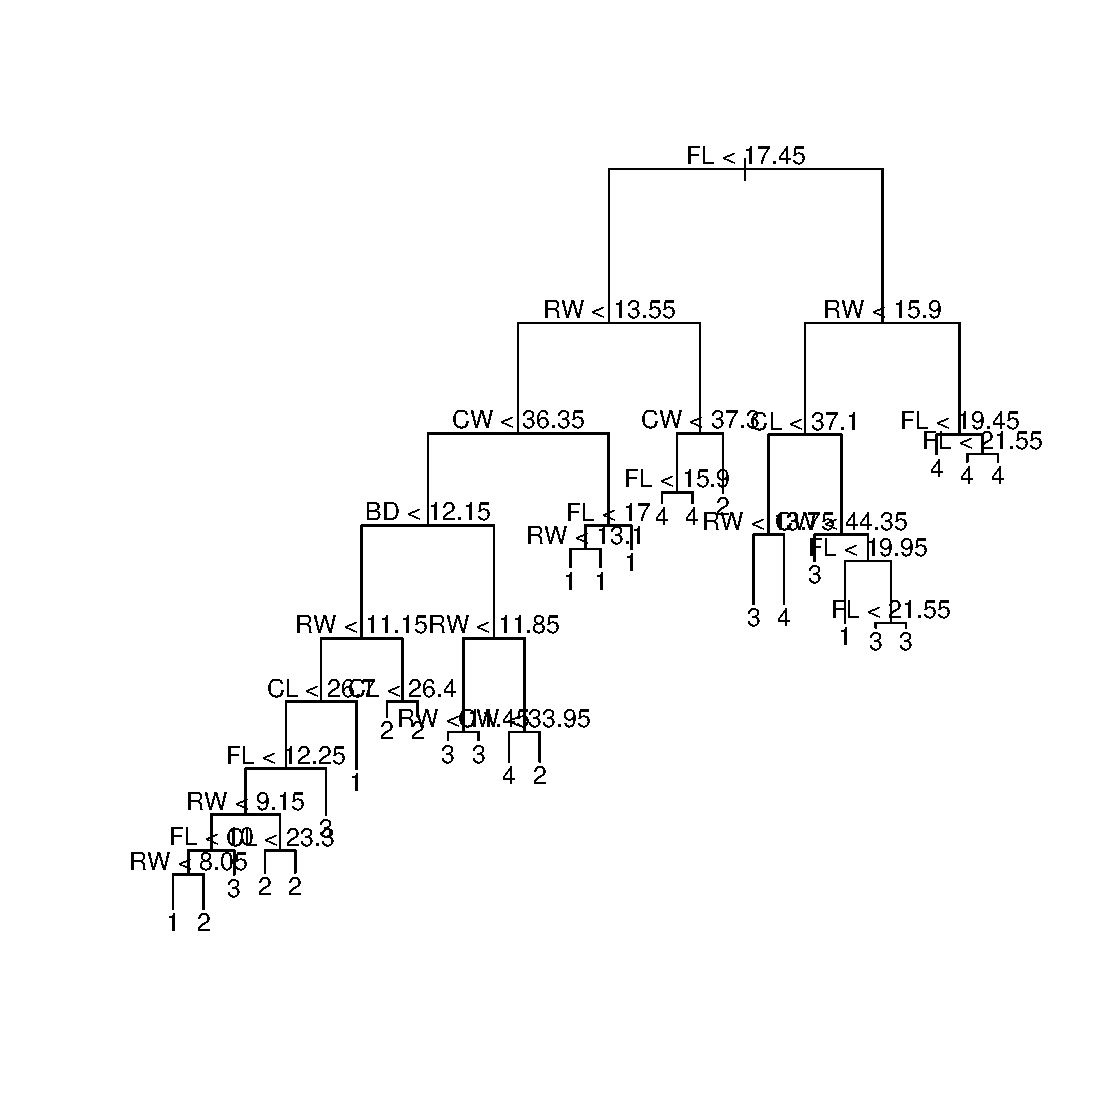
\includegraphics[width=.32\textwidth]{oblique_splits_crabs_original_off_tree.ps}
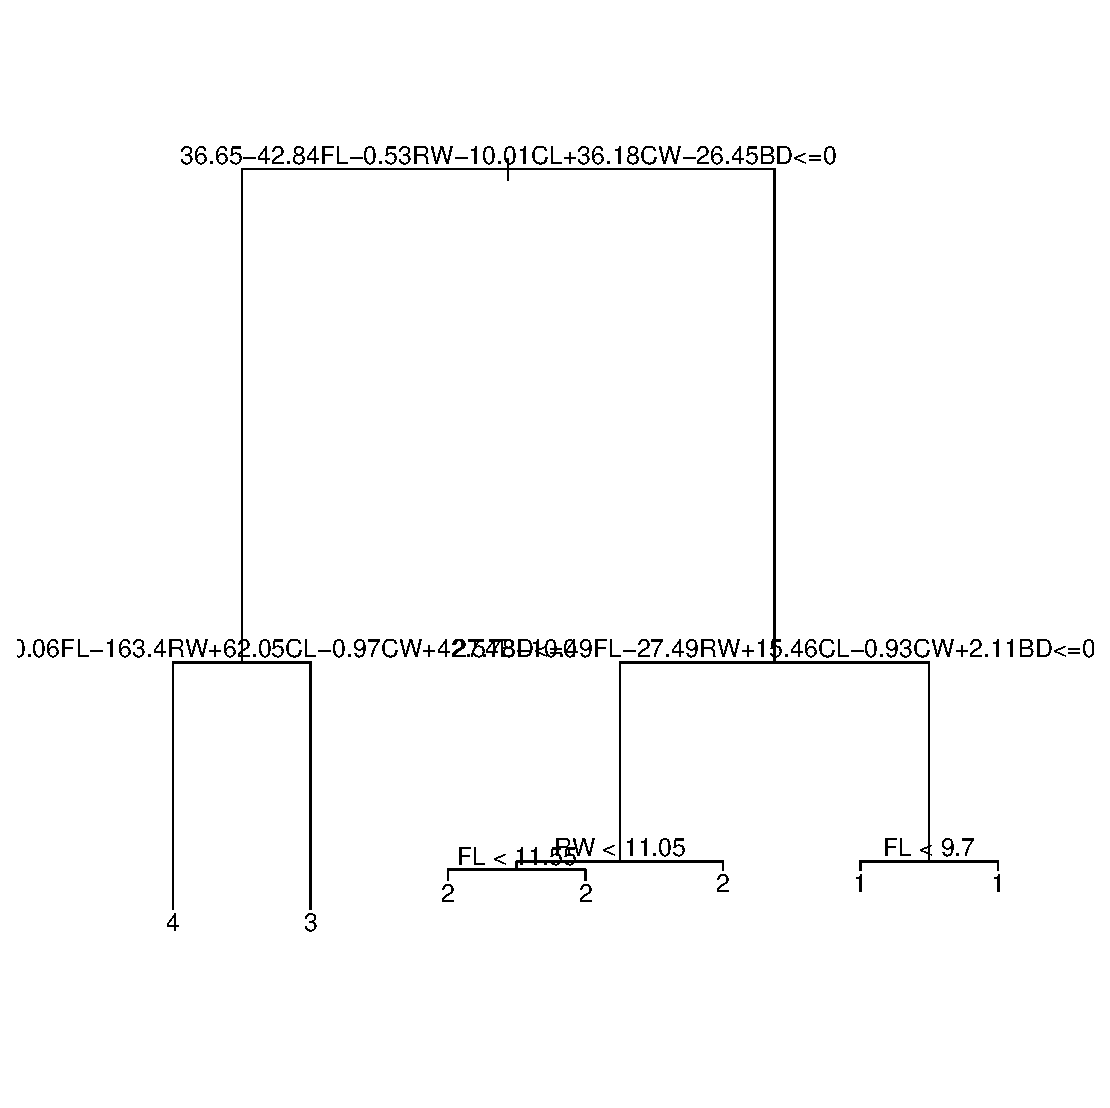
\includegraphics[width=.32\textwidth]{oblique_splits_crabs_original_on_tree.ps}
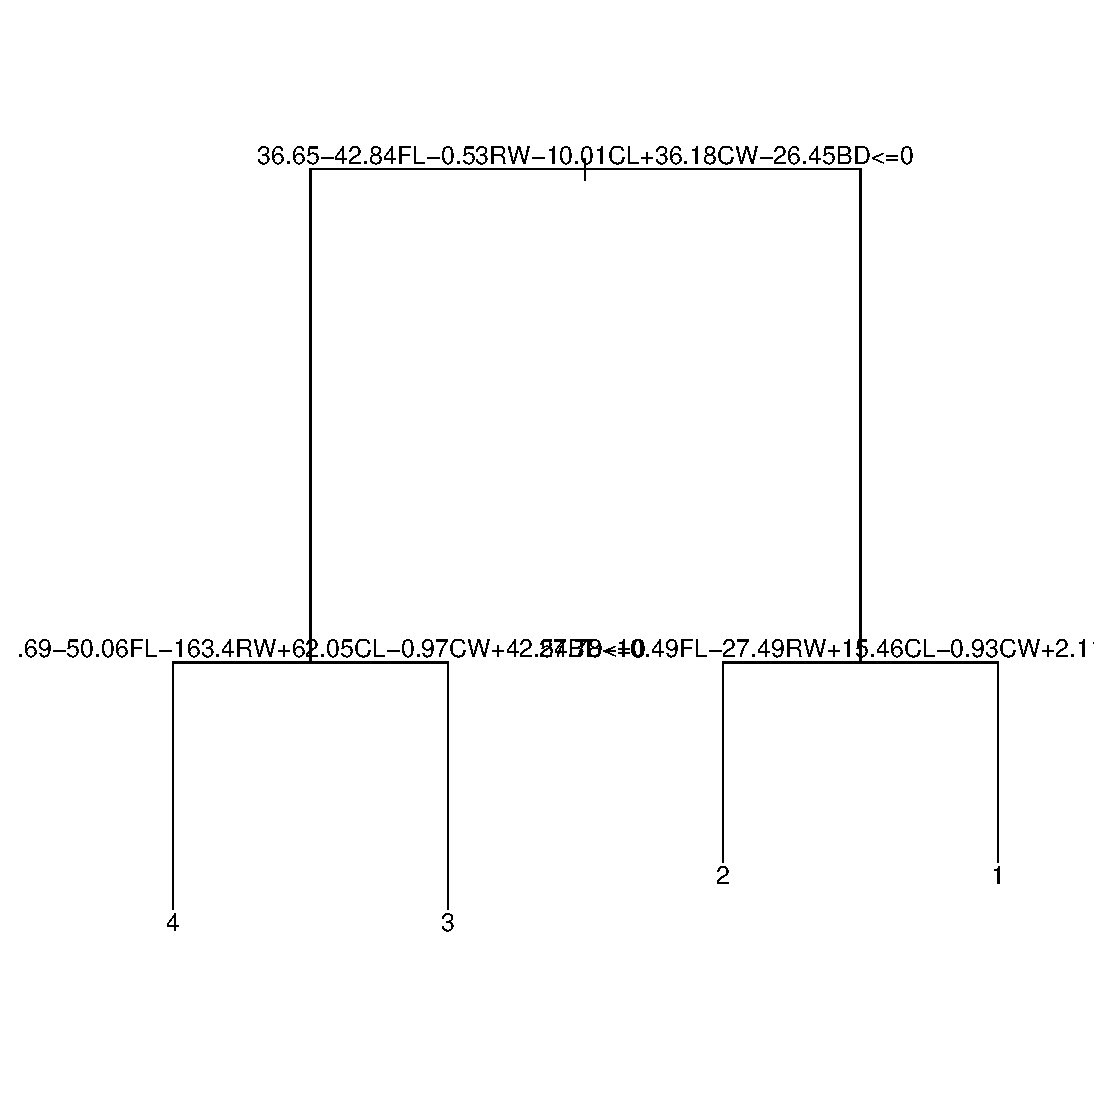
\includegraphics[width=.32\textwidth]{oblique_splits_crabs_original_only_tree.ps}
\caption{Axis-parallel tree, mixture tree and oblique tree grown on original crabs dataset}
\label{fig:oblique_splits_crabs_original}
\end{figure}

It is known that observations of different classes are well separated by oblique splits in this dataset. The axis-parallel tree grown is rather large as requires concatentated use of axis-parallel splits to partition observations. Allowing oblique splits, mixture trees and oblique trees use oblique splits to produce large reductions in deviance. \\

It should also be noted that when using oblique splits exclusively, only 7 (=$2^{4-1}-1$) splits need to be evaluated at the root node as compared to the 995 odd ($\approx(200-1)\times 5$) in the case of axis-parallel trees.

\subsection{Augmented Crabs Data}
\label{AugmentedCrabsData}
By projecting the crabs dataset onto its principal components second and third principal components, observations of different classes are much better separated. Axis-parallel trees should perform better on this \emph{Augmented Crabs dataset} as a result. With a 2-dimensional dataset, it is also possible to view the decision boundaries of each tree as is shown in Figures~\ref{fig:oblique_splits_crabs_augmented_off}-~\ref{fig:oblique_splits_crabs_augmented_only}.\\

\begin{figure}
\centering
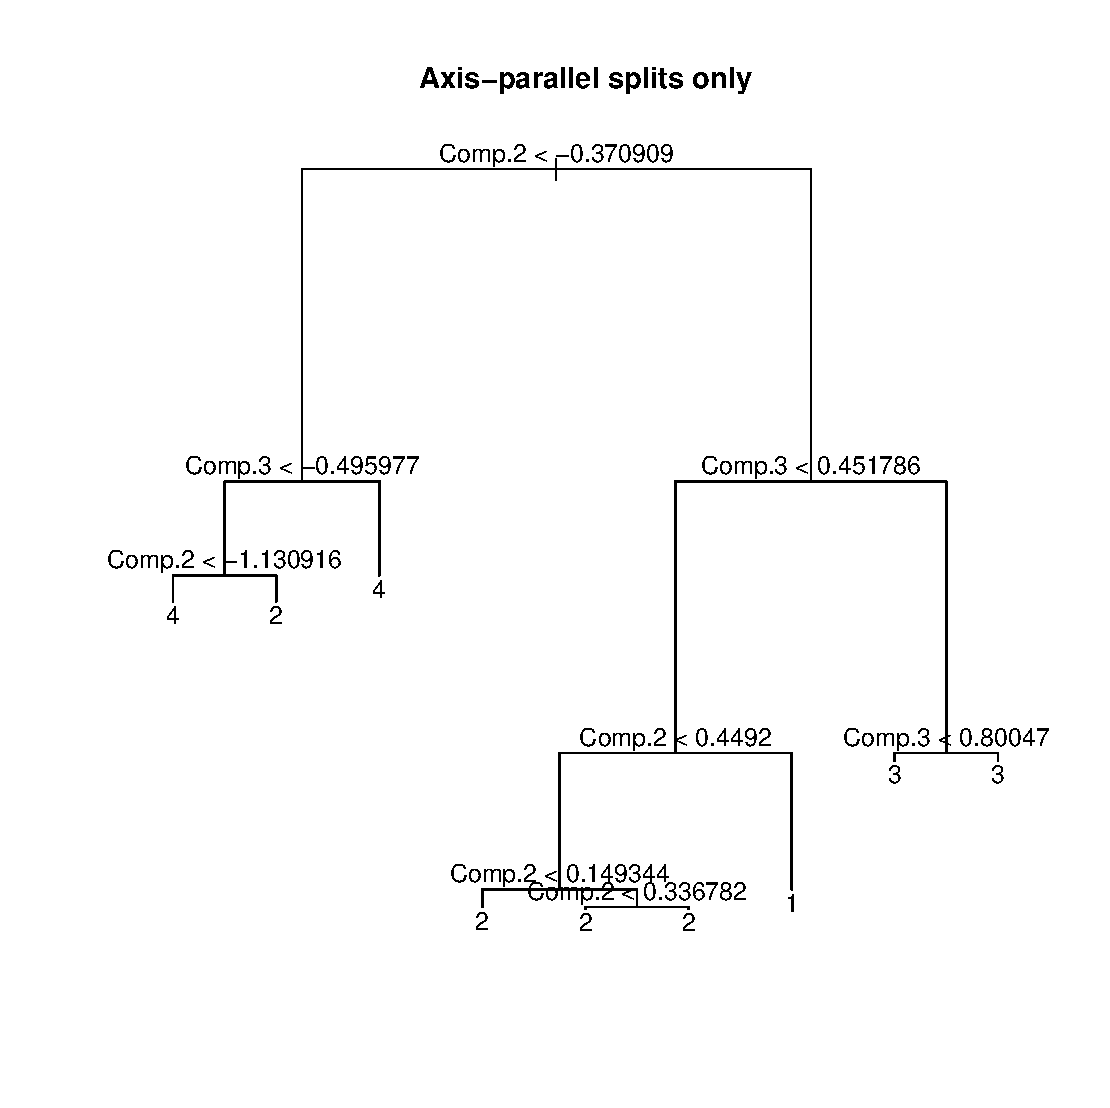
\includegraphics[width=.4\textwidth]{oblique_splits_crabs_augmented_off_tree.ps}
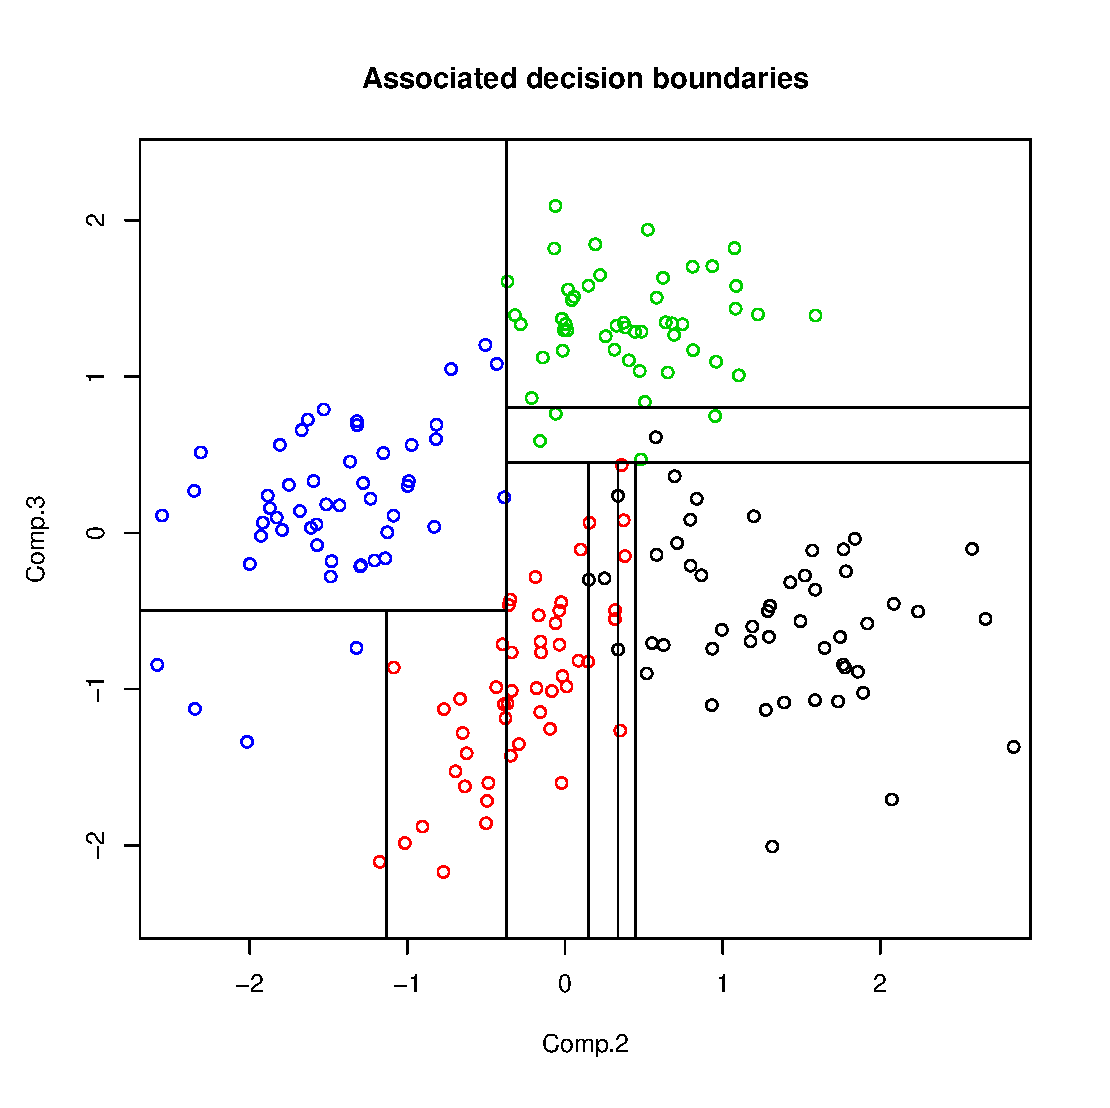
\includegraphics[width=.4\textwidth]{oblique_splits_crabs_augmented_off_decision_boundaries.ps}
\caption{Axis-parallel tree grown on the Augmented Crabs dataset with its associated decision boundaries}
\label{fig:oblique_splits_crabs_augmented_off}
\end{figure}
\begin{figure}
\centering
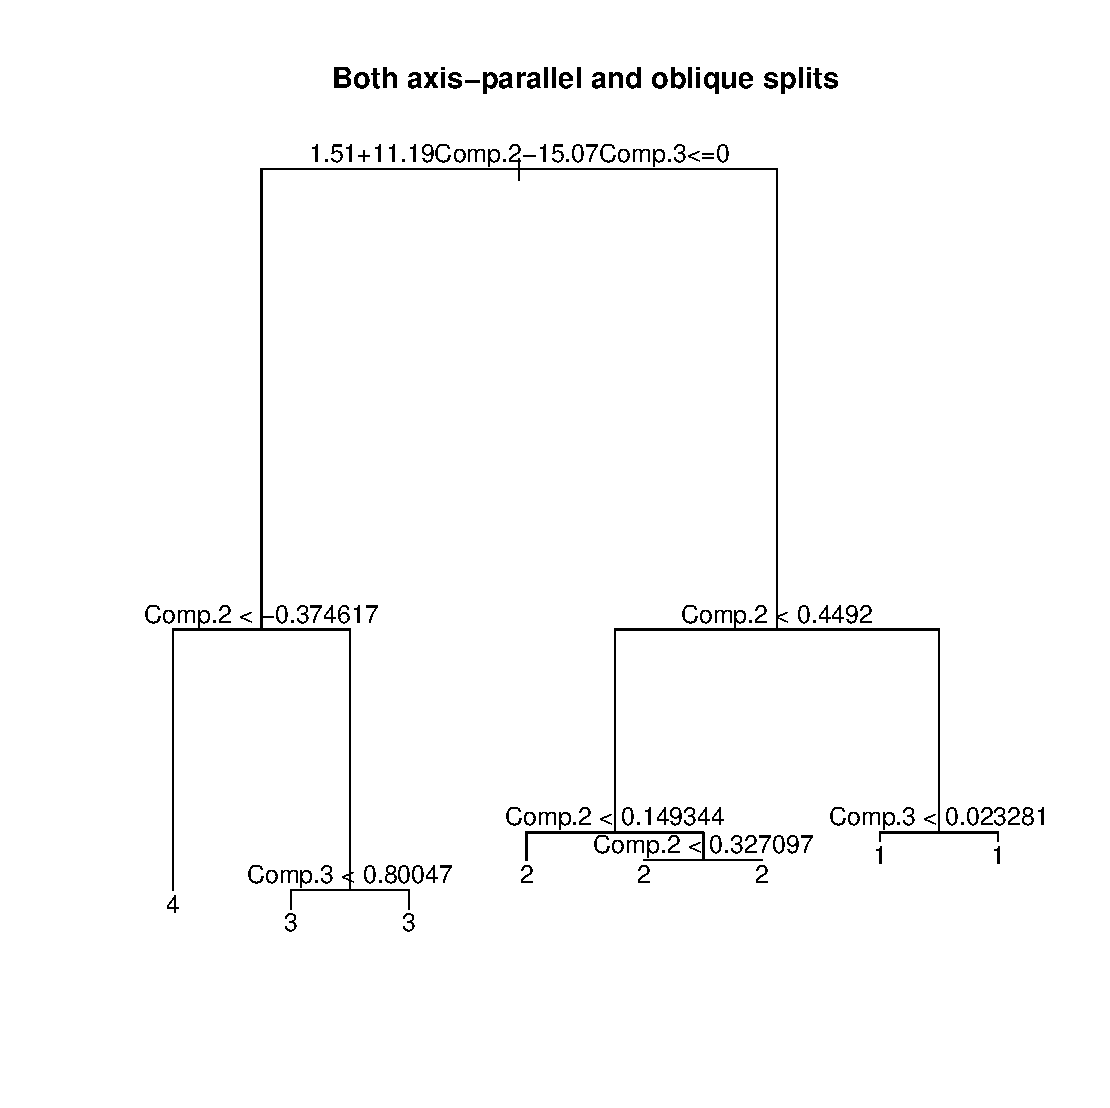
\includegraphics[width=.4\textwidth]{oblique_splits_crabs_augmented_on_tree.ps}
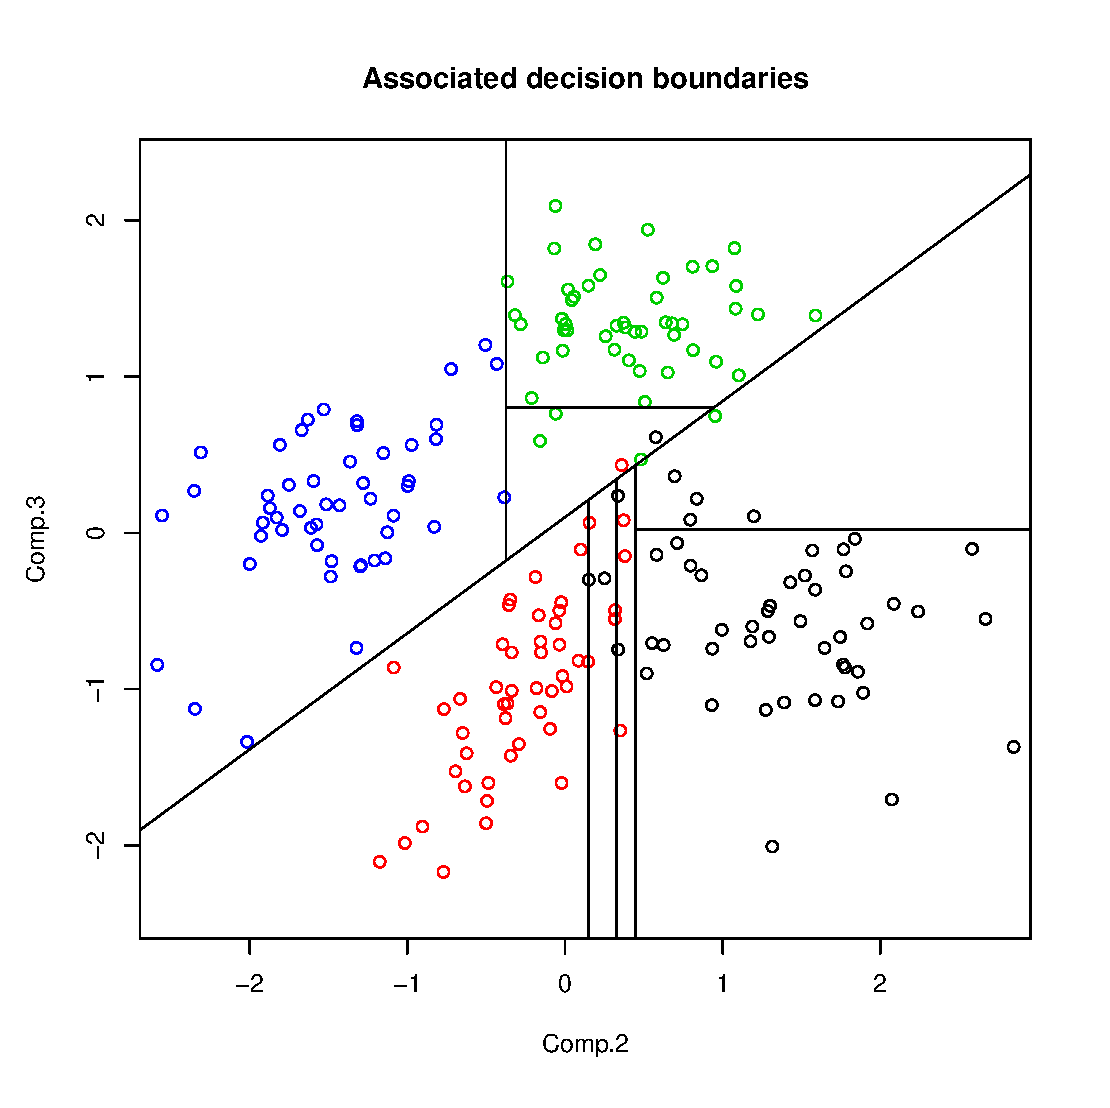
\includegraphics[width=.4\textwidth]{oblique_splits_crabs_augmented_on_decision_boundaries.ps}
\caption{Mixture tree grown on the Augmented Crabs dataset with its associated decision boundaries}
\label{fig:oblique_splits_crabs_augmented_on}
\end{figure}
\begin{figure}
\centering
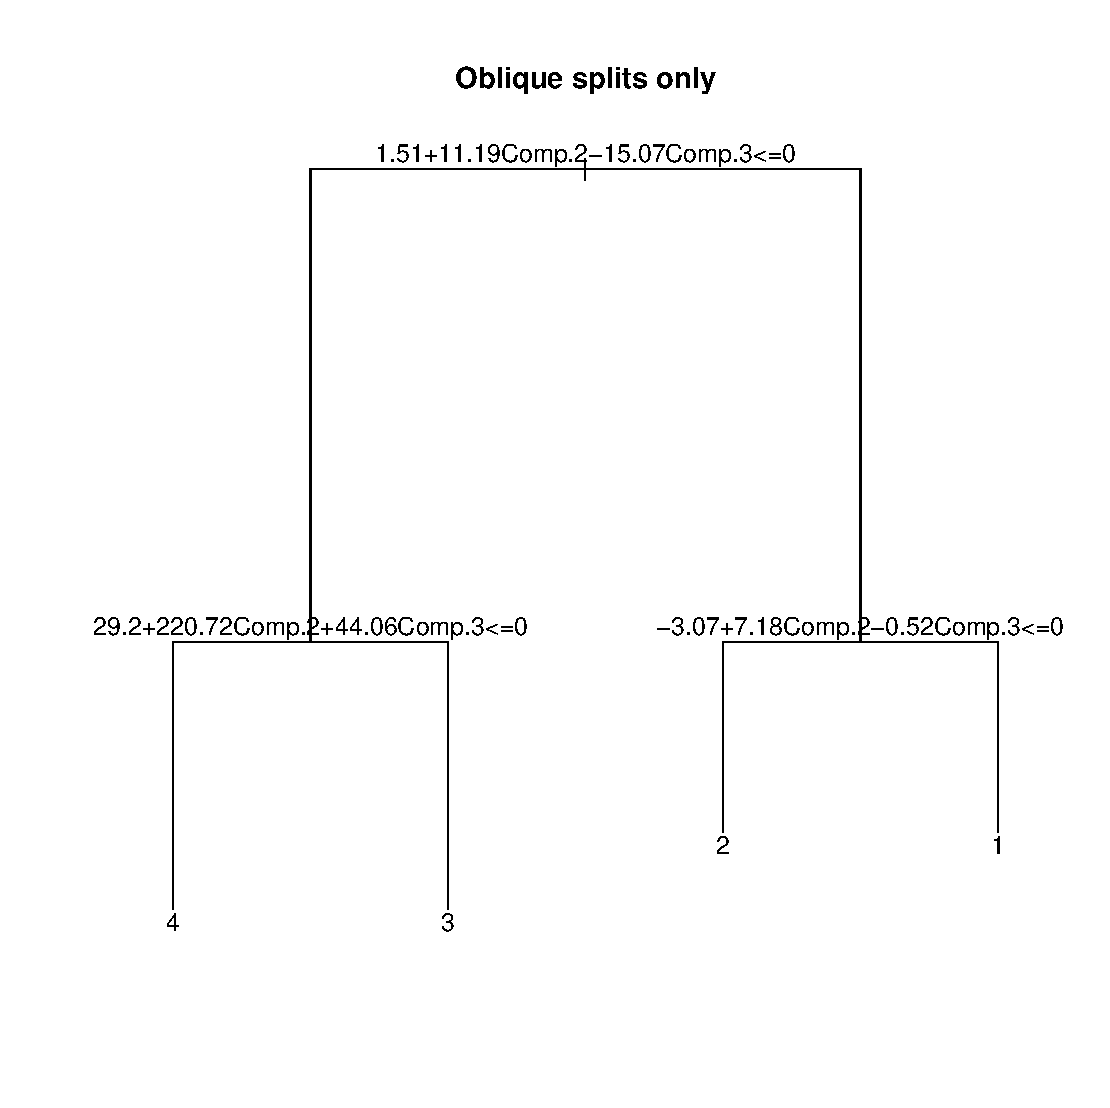
\includegraphics[width=.4\textwidth]{oblique_splits_crabs_augmented_only_tree.ps}
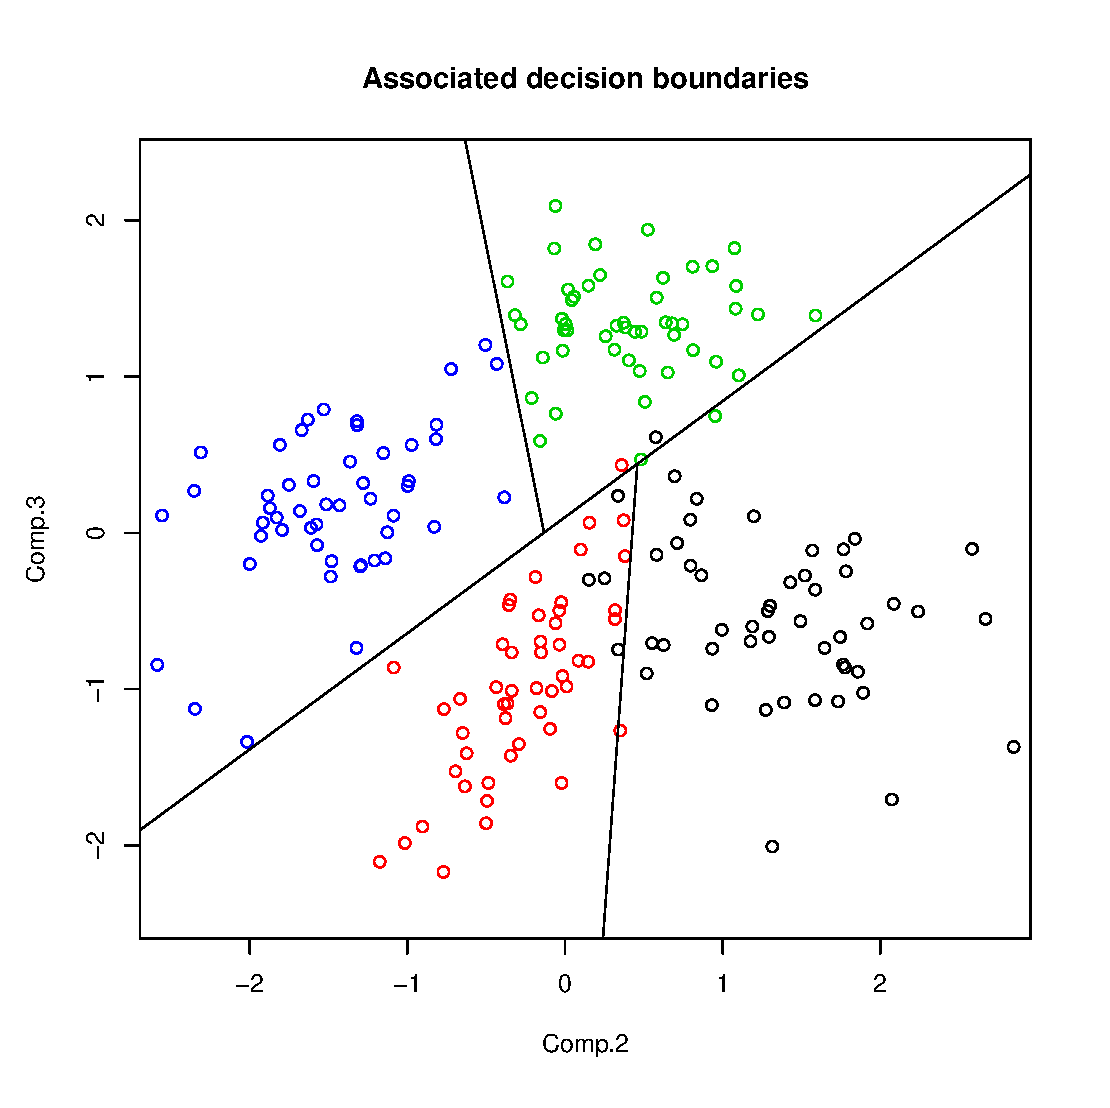
\includegraphics[width=.4\textwidth]{oblique_splits_crabs_augmented_only_decision_boundaries.ps}
\caption{Oblique tree grown on the Augmented Crabs dataset with its associated decision boundaries}
\label{fig:oblique_splits_crabs_augmented_only}
\end{figure}

Looking at the trees, the axis-parallel tree is indeed smaller than the one grown on the original crabs dataset however when compared to mixture and oblique trees, it still uses more tests. By examining decision boundaries of each tree, it is easy to see why. Observations are best partitioned with oblique splits.

\subsection{Pima Indians Data}
\label{PimaIndiansData}
The Pima Indians dataset contains 7 measurements from 532 women of Pima Indian heritage living near Pheonix, Arizona tested for the presence (or lackthereof) of diabetes. A subset containing 200 observations called \texttt{Pima.tr} found in the \emph{Modern Applied Statistics with S-Plus} library in R is used as the training set. Trees grown on this dataset are shown in Figure~\ref{fig:oblique_splits_pima_trees} both with and without text for greater clarity.\\

\begin{figure}
\centering
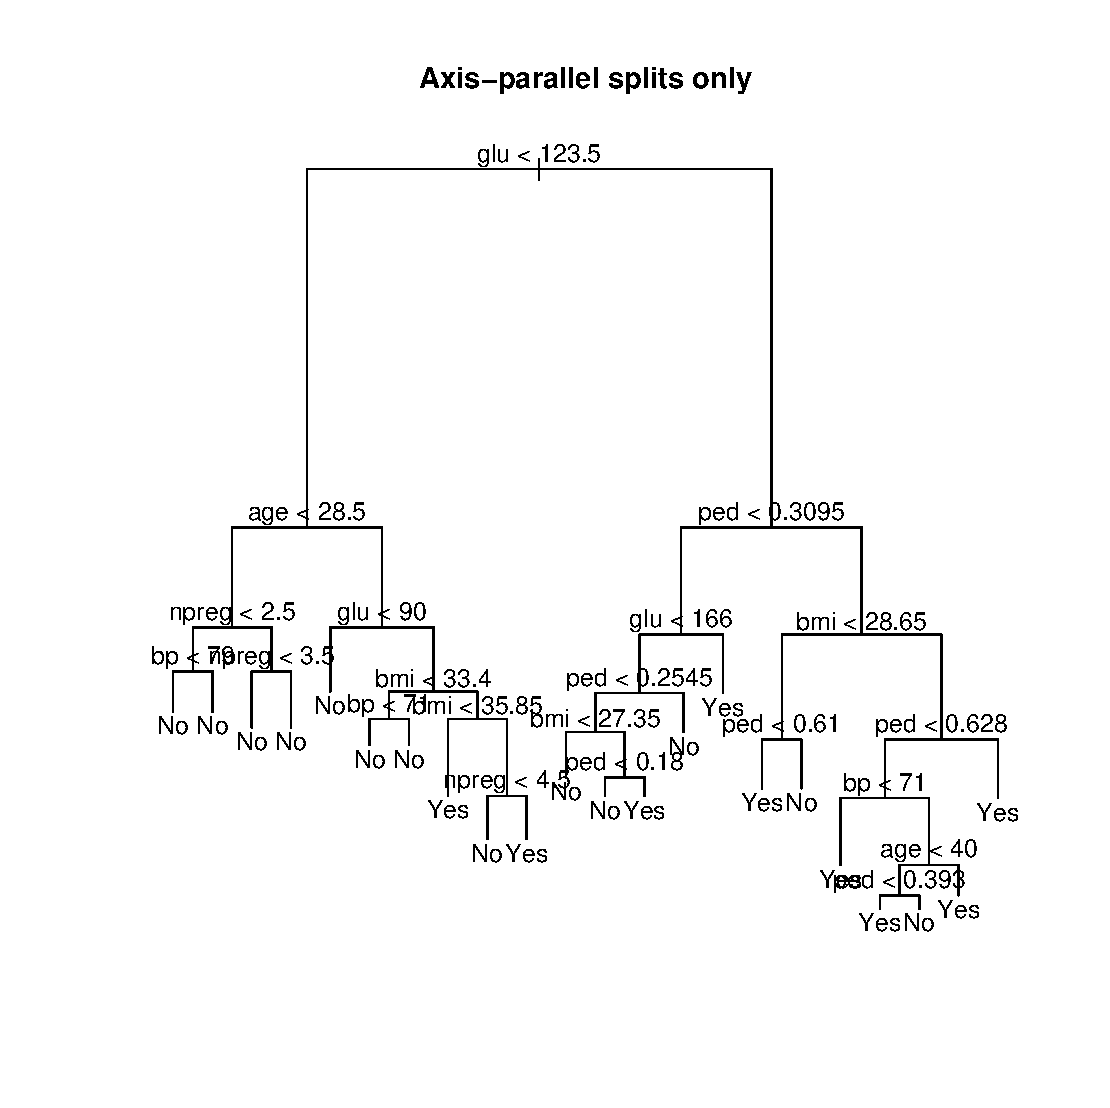
\includegraphics[width=.32\textwidth]{oblique_splits_pima_off_tree.ps}
\includegraphics[width=.32\textwidth]{oblique_splits_pima_on_tree.ps}
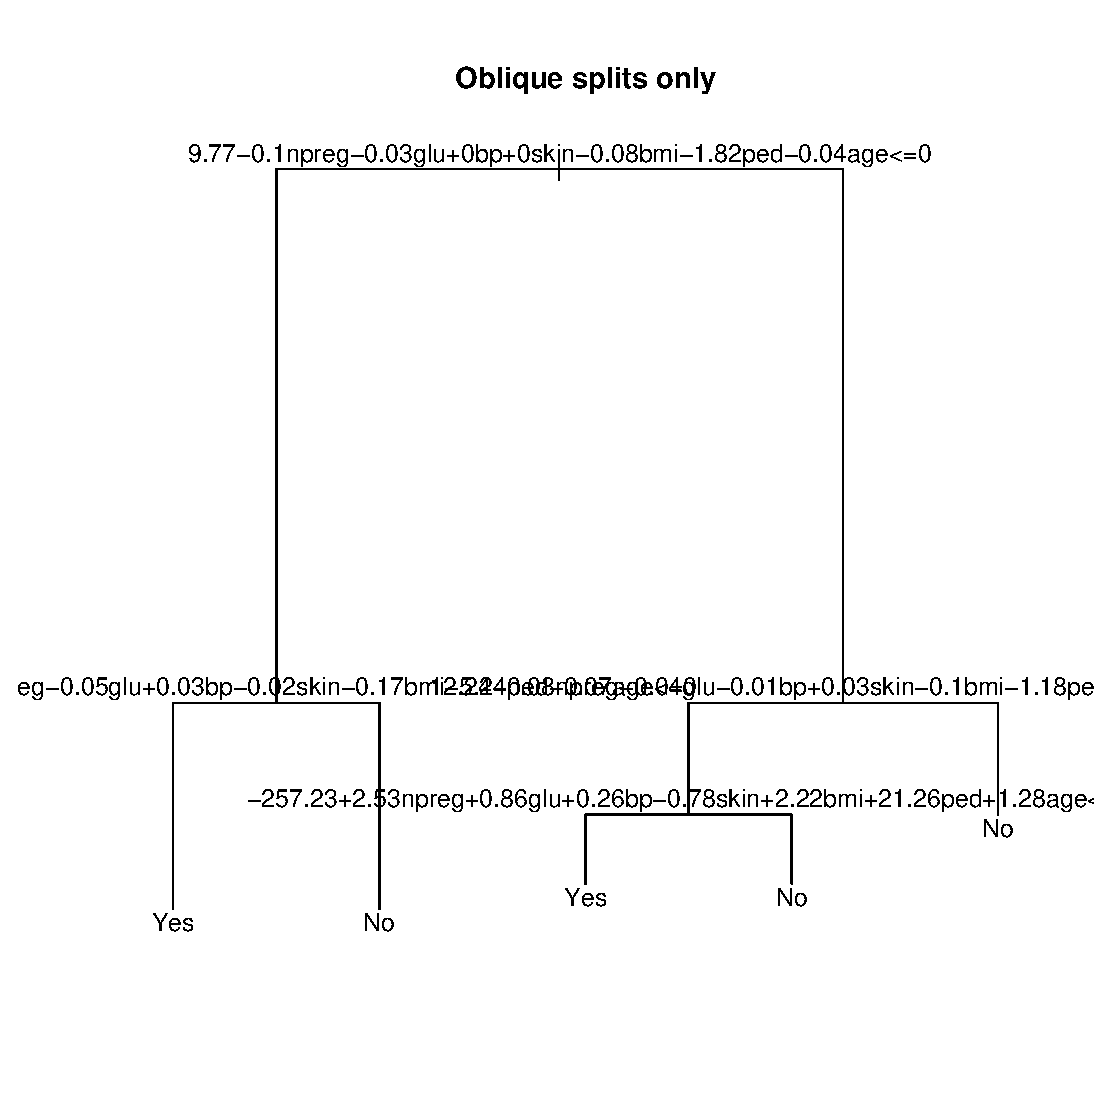
\includegraphics[width=.32\textwidth]{oblique_splits_pima_only_tree.ps}\\
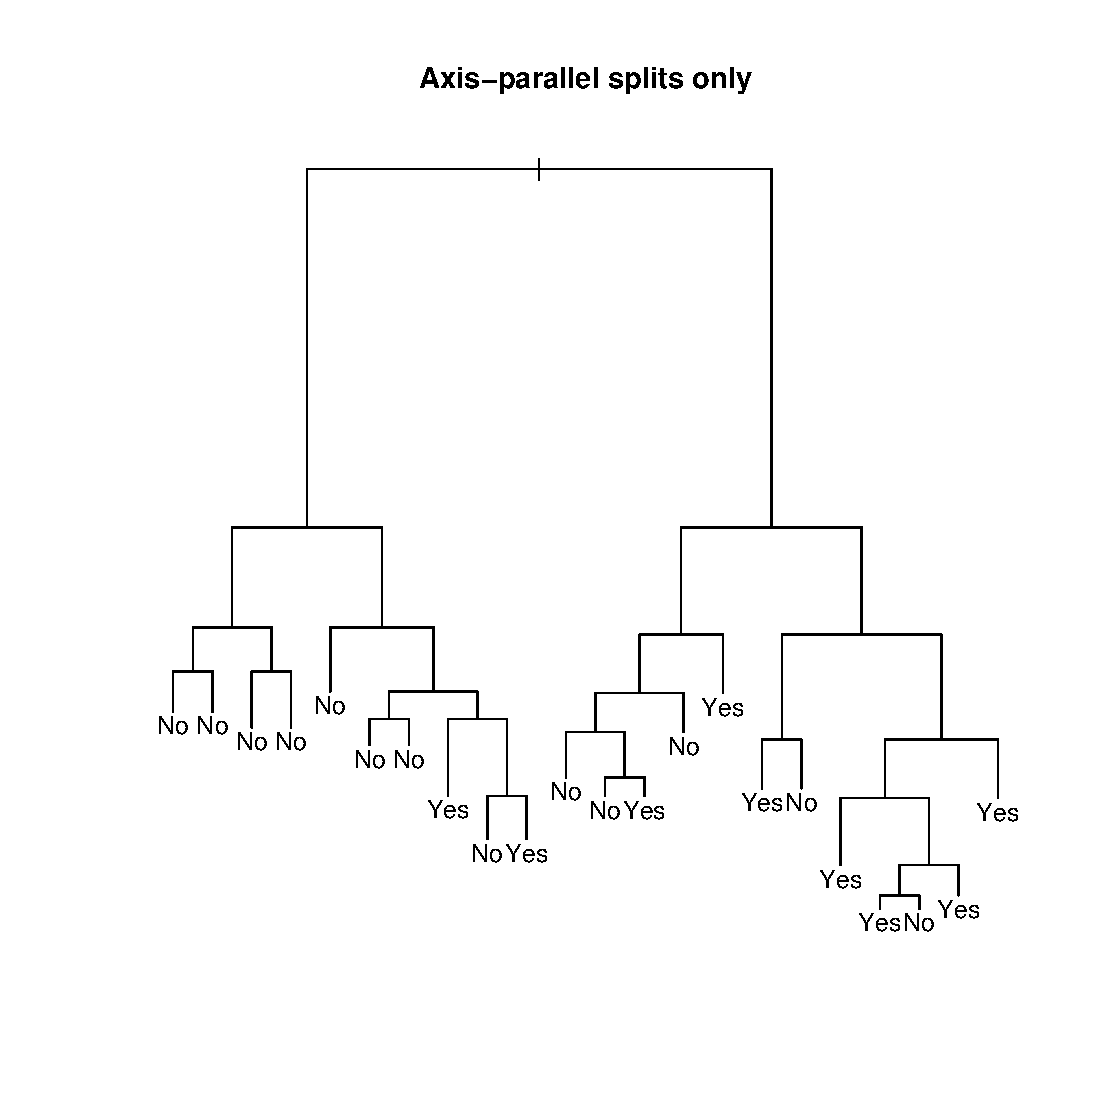
\includegraphics[width=.32\textwidth]{oblique_splits_pima_off_tree_skeleton.ps}
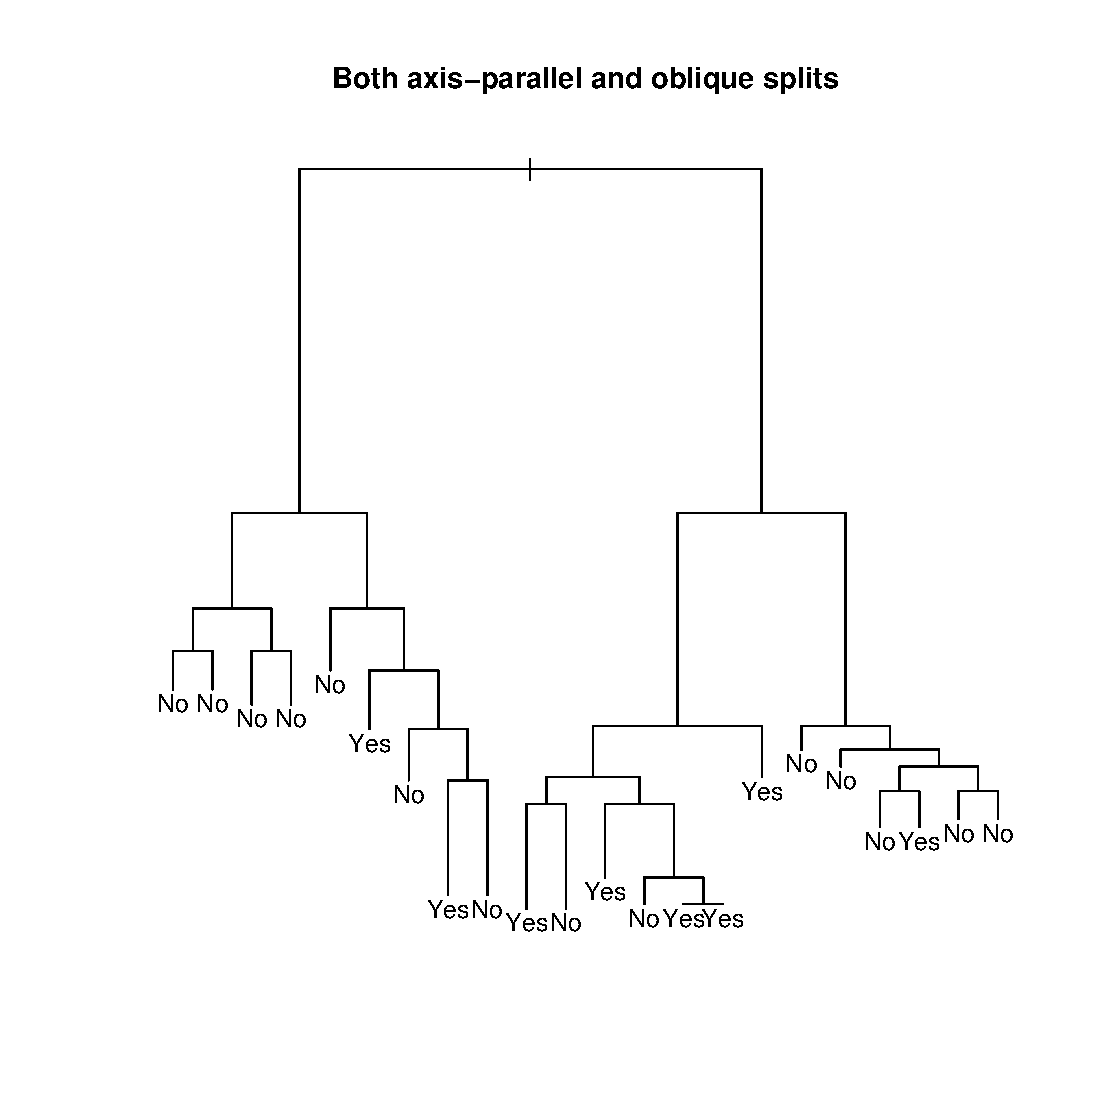
\includegraphics[width=.32\textwidth]{oblique_splits_pima_on_tree_skeleton.ps}
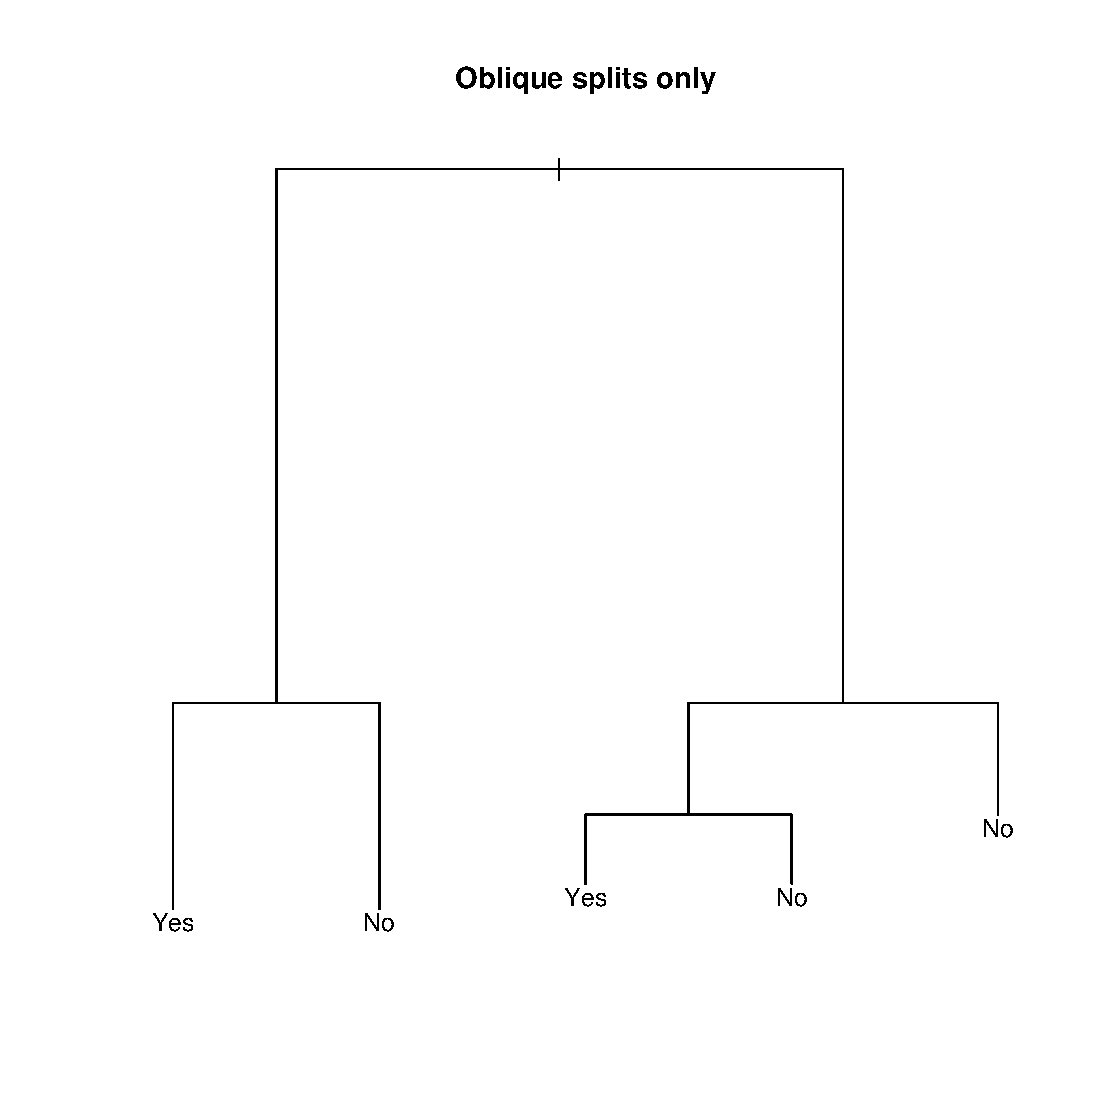
\includegraphics[width=.32\textwidth]{oblique_splits_pima_only_tree_skeleton.ps}
\caption{Trees grown on the Pima Indians dataset and their associated tree skeletons}
\label{fig:oblique_splits_pima_trees}
\end{figure}

As with before, much few tests are used when oblique splits are used.\\

\subsection{Glass Fragments Data}
\label{GlassFragmentsData}
The same can be said for the Glass Fragments dataset.
\begin{figure}
\centering
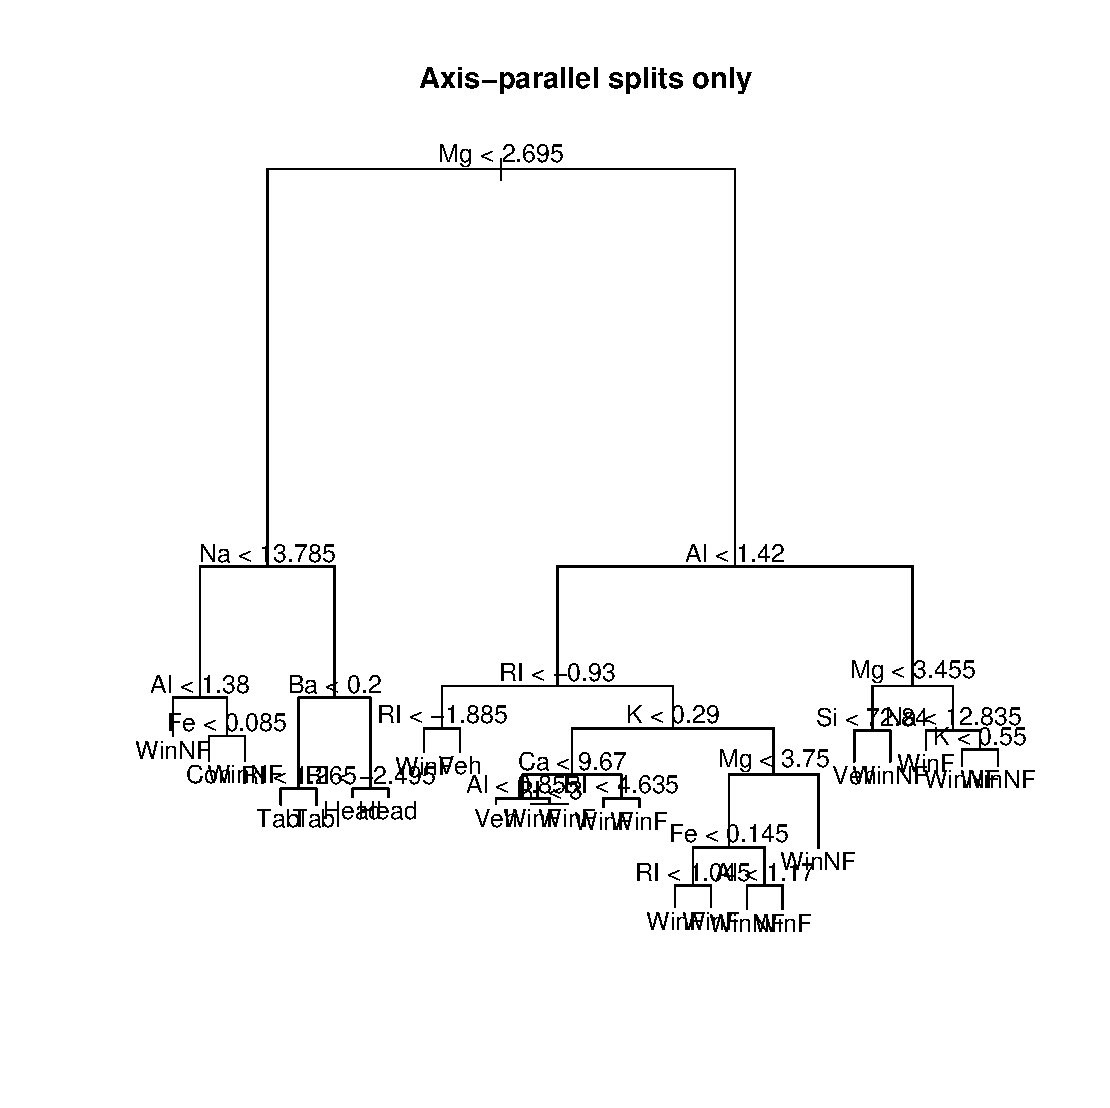
\includegraphics[width=.32\textwidth]{oblique_splits_fgl_off_tree.ps}
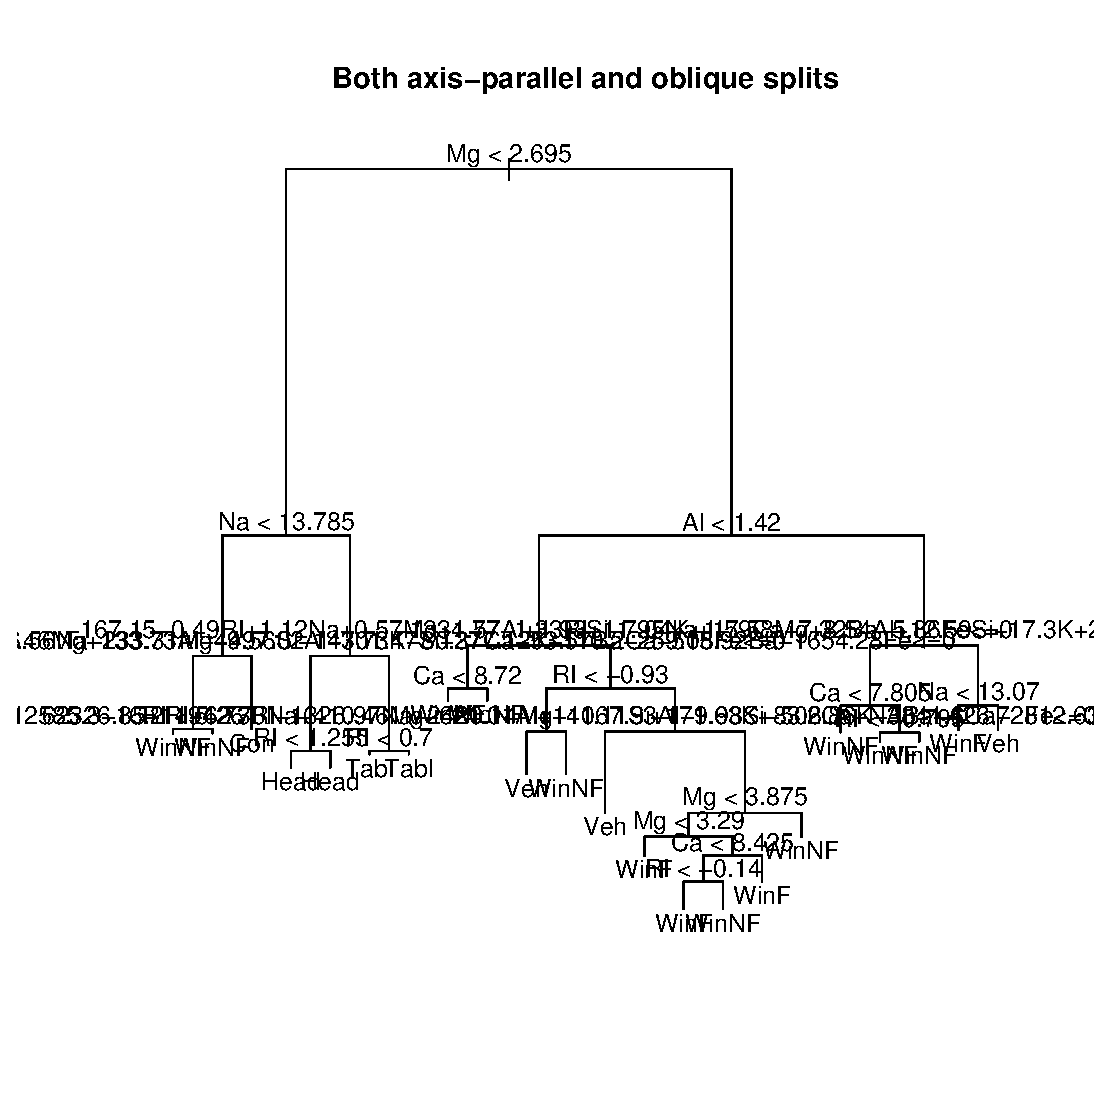
\includegraphics[width=.32\textwidth]{oblique_splits_fgl_on_tree.ps}
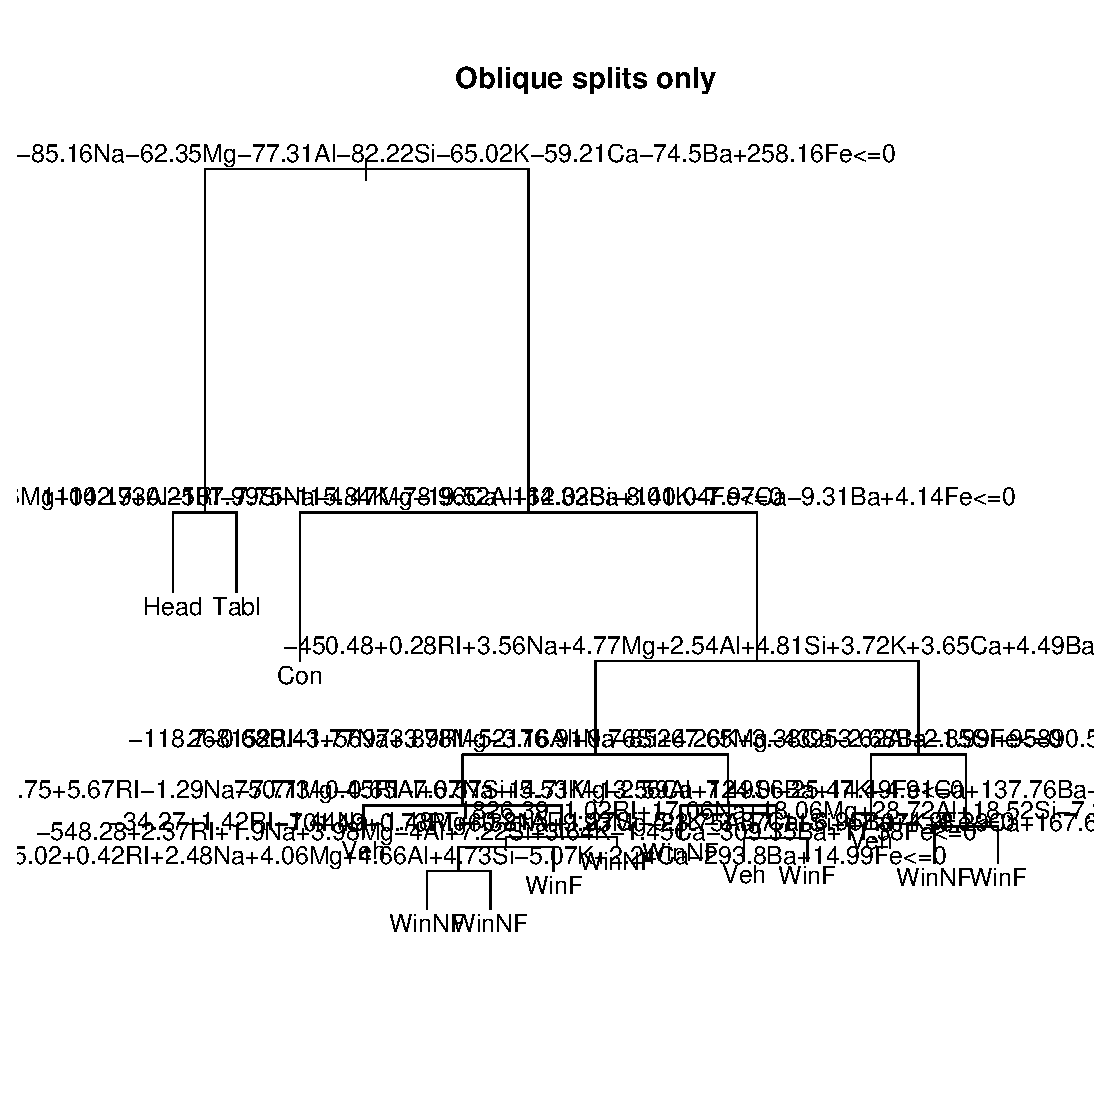
\includegraphics[width=.32\textwidth]{oblique_splits_fgl_only_tree.ps}\\
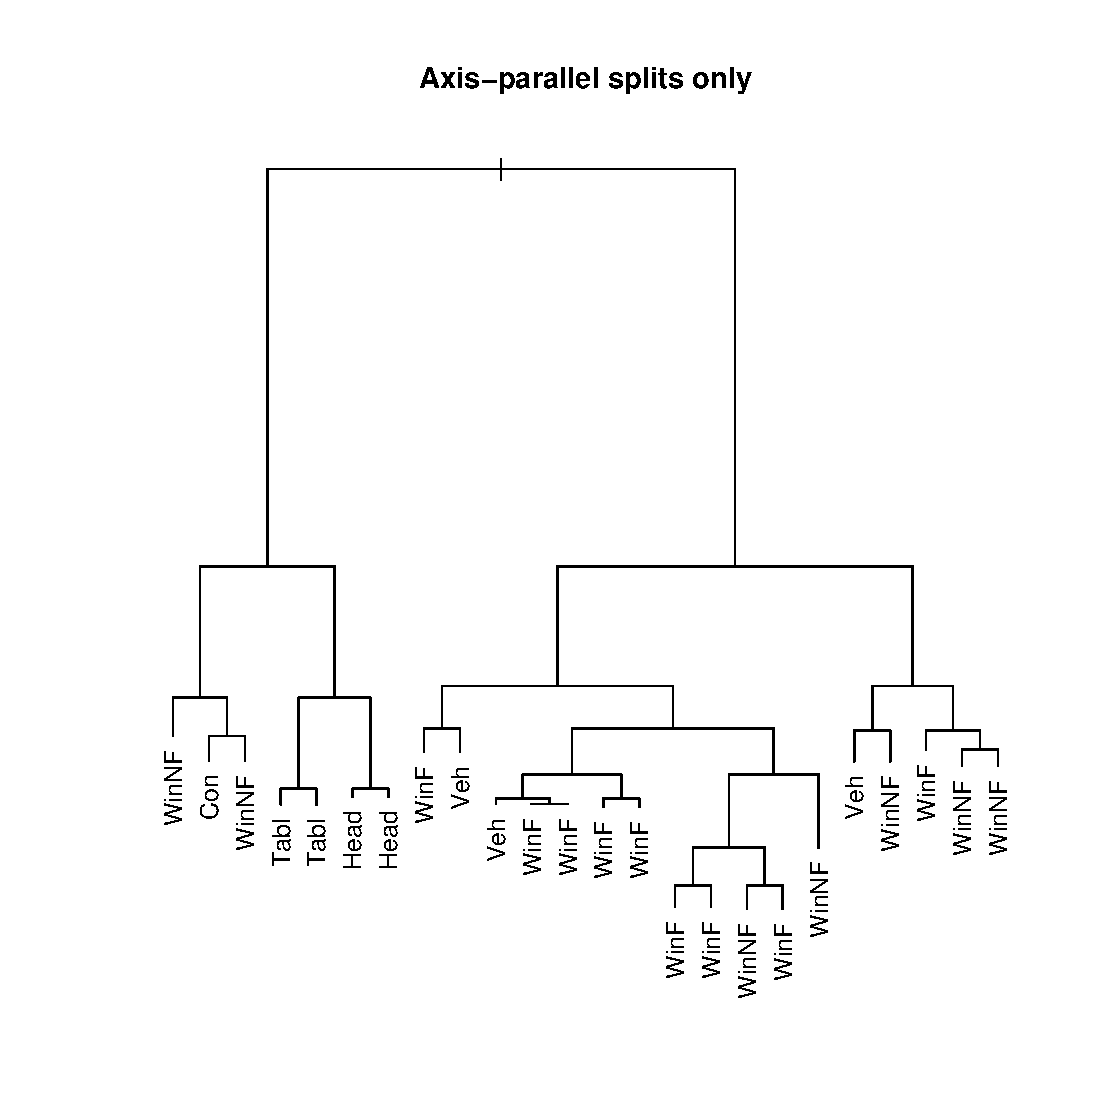
\includegraphics[width=.32\textwidth]{oblique_splits_fgl_off_tree_skeleton.ps}
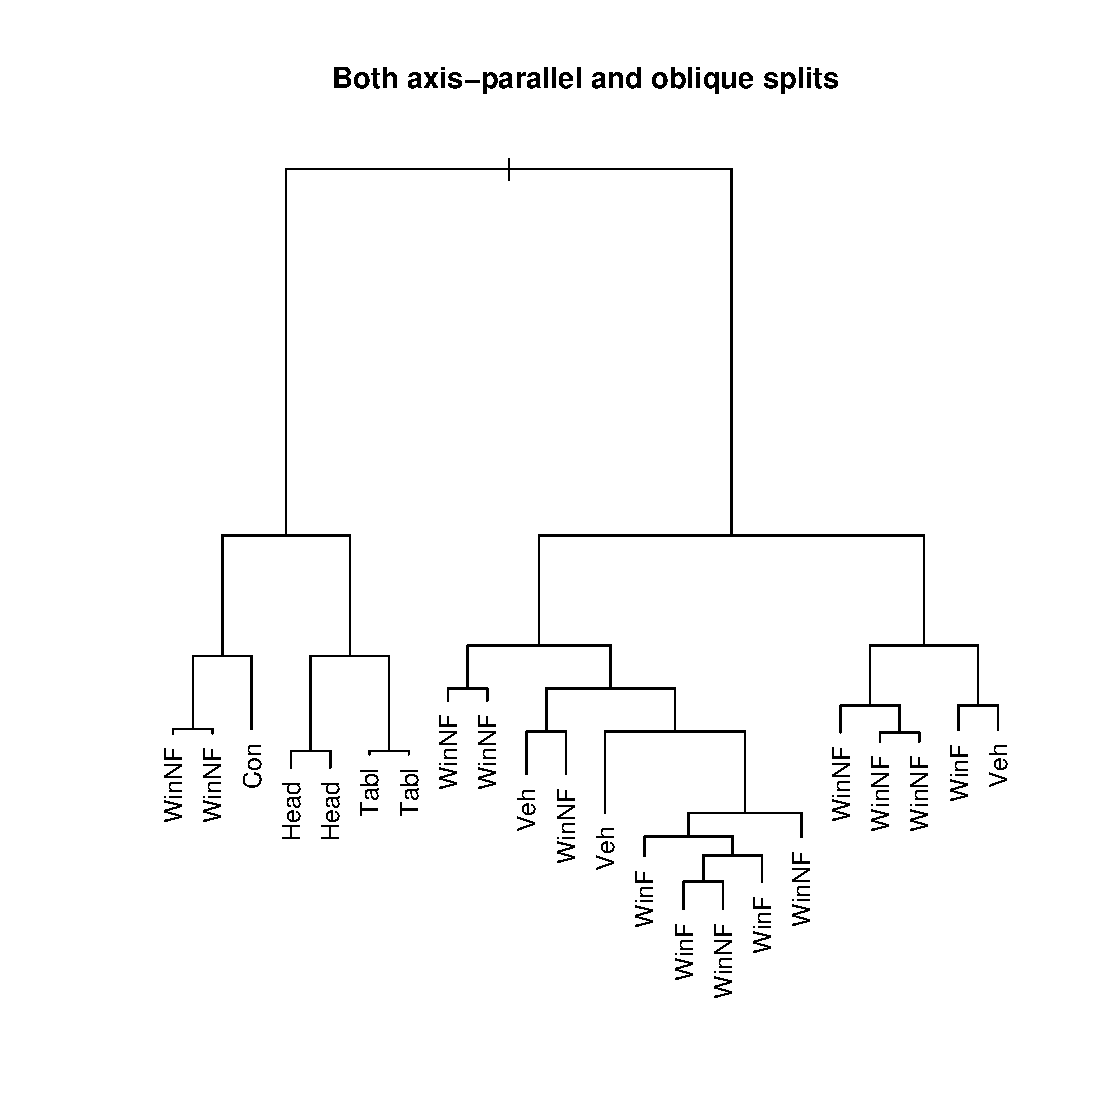
\includegraphics[width=.32\textwidth]{oblique_splits_fgl_on_tree_skeleton.ps}
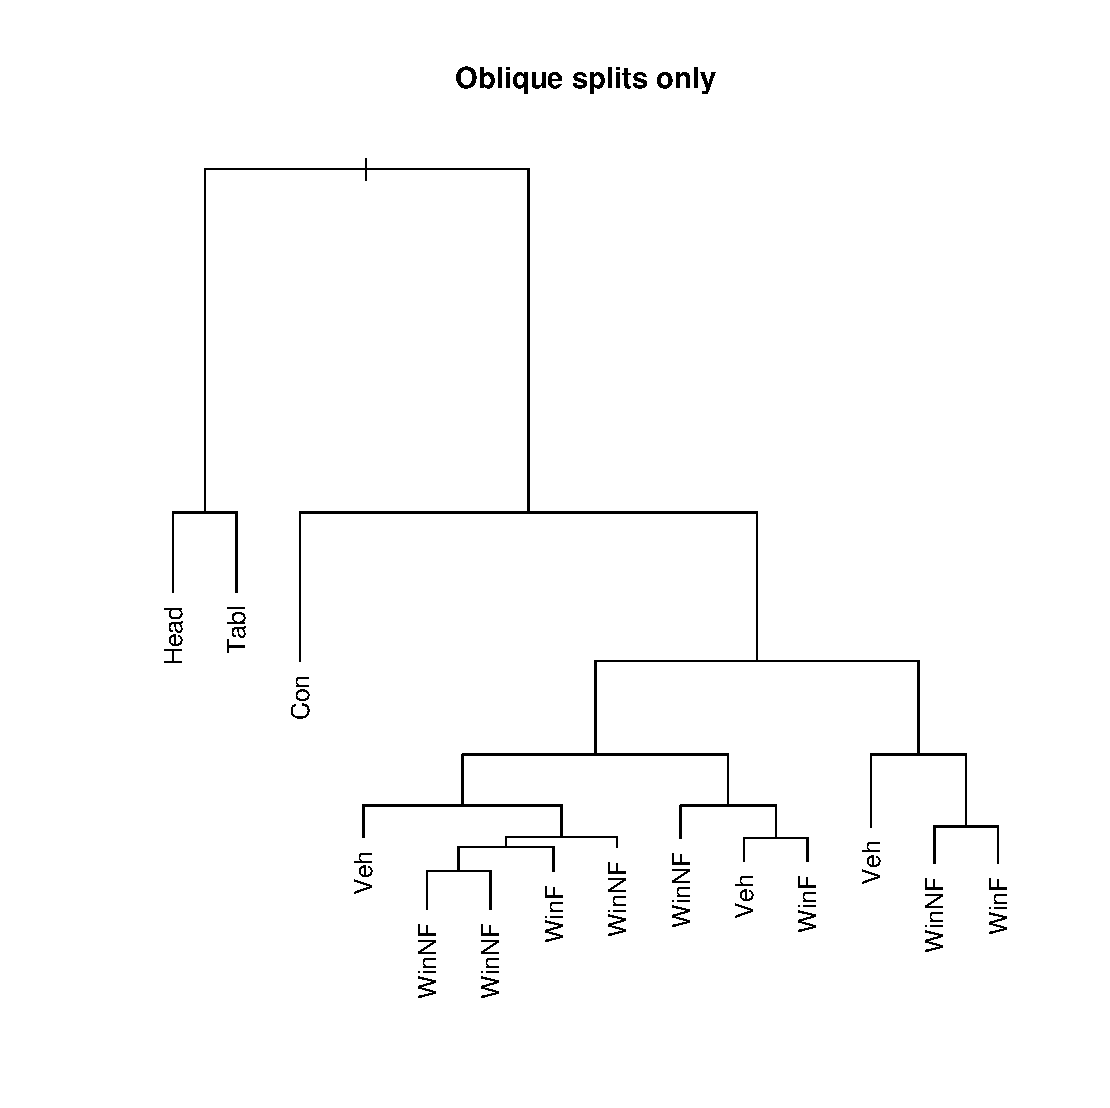
\includegraphics[width=.32\textwidth]{oblique_splits_fgl_only_tree_skeleton.ps}
\caption{Trees grown on the Glass Fragments dataset and their associated tree skeletons}
\label{fig:oblique_splits_fgl_tree}
\end{figure}

\section{Locally Optimal Subset}
\label{LocallyOptimalSubset}
The family of oblique splits specified in Section~\ref{IdealOutcomes} is intuitively appealing and as Section~\ref{ExamplesofObliqueTrees} shows allows interesting oblique trees to be grown. With an oblique split dictionary of size $\sum_{k=0}^{q} {L_{gen}-1\choose k}-1$ it is surprising how a subset of size $2^{R-1}-1$ can perform so well. A heuristic argument follows seeking to explain why much of the oblique split dictionary can be ignored with empirical evidence to back this claim. \\

As previously noted, widely used methods of tree growth seek to apply the best split at each stage. The impurity of every split in the split dictionary must be considered to do this. It is easy to see that most splits produce similar outcomes over continuous attributes and so many splits are evaluated unnecessarily. Contains splits that produce all possible partitioning of observations to child nodes, some splits differ by only an observation or two (in its child nodes) are considered separate splits in the split dictionary. Such splits are said to be \emph{similar} and it follows that their impurities are also very similar. Just how many similar splits are there in the axis-parallel and oblique split dictionaries?\\

For any given axis-parallel split $X_i=c$, increasing (or decreasing) $c$ to the next unique value of $X_i$ in the training set can result in a similar split (failing to hold only when many observations take the same value of $X_i$). There are therefore around 2 similar splits for any given axis-parallel split. The evolution of the impurity measure over a typical training sets are shown in Figure~\ref{fig:impurity_plot_1d}.\\

\begin{figure}
\centering
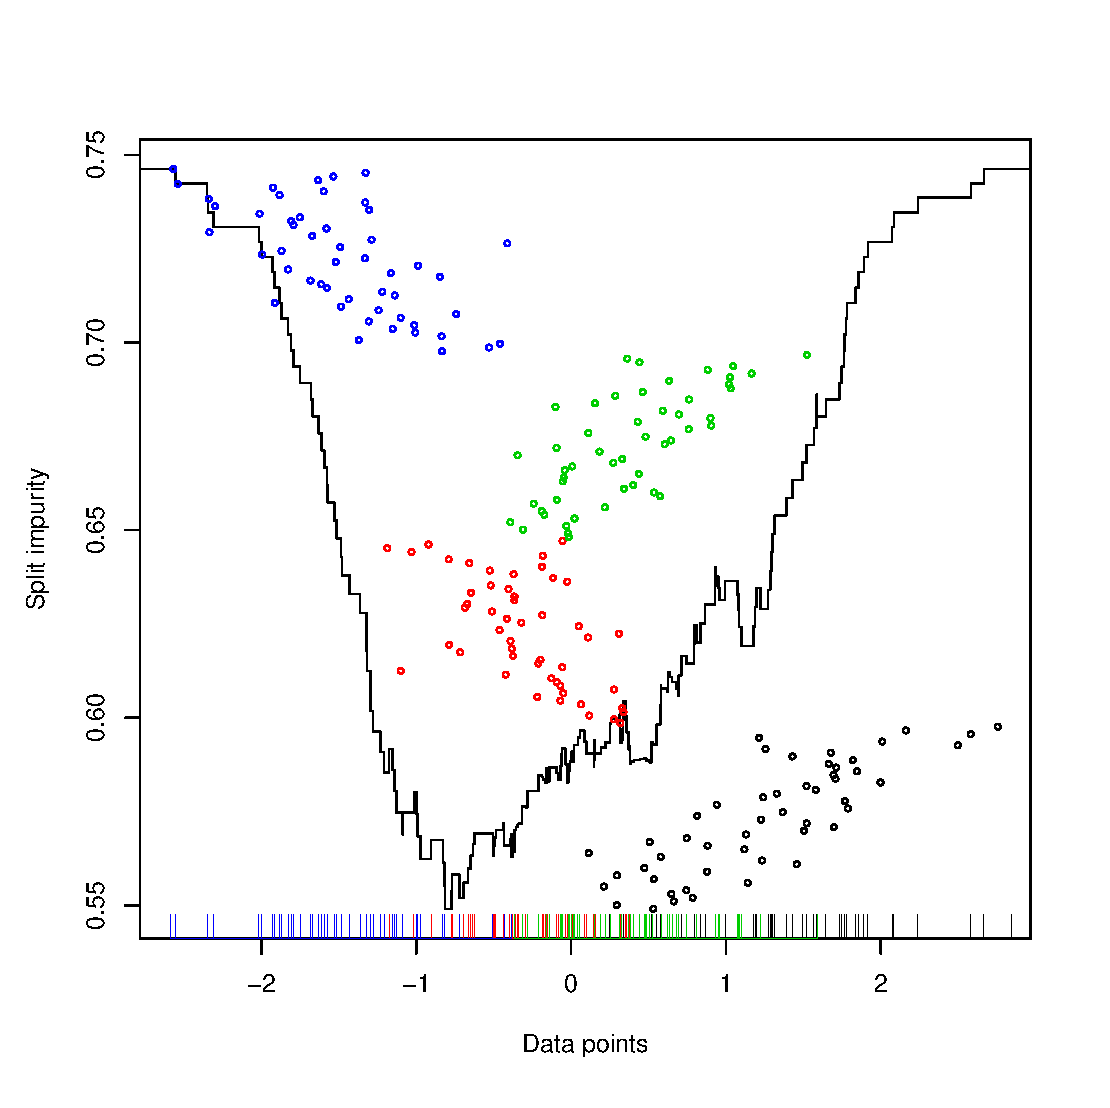
\includegraphics[width=.49\textwidth]{impurity_plot_1d_crabs_data_pc2.ps}
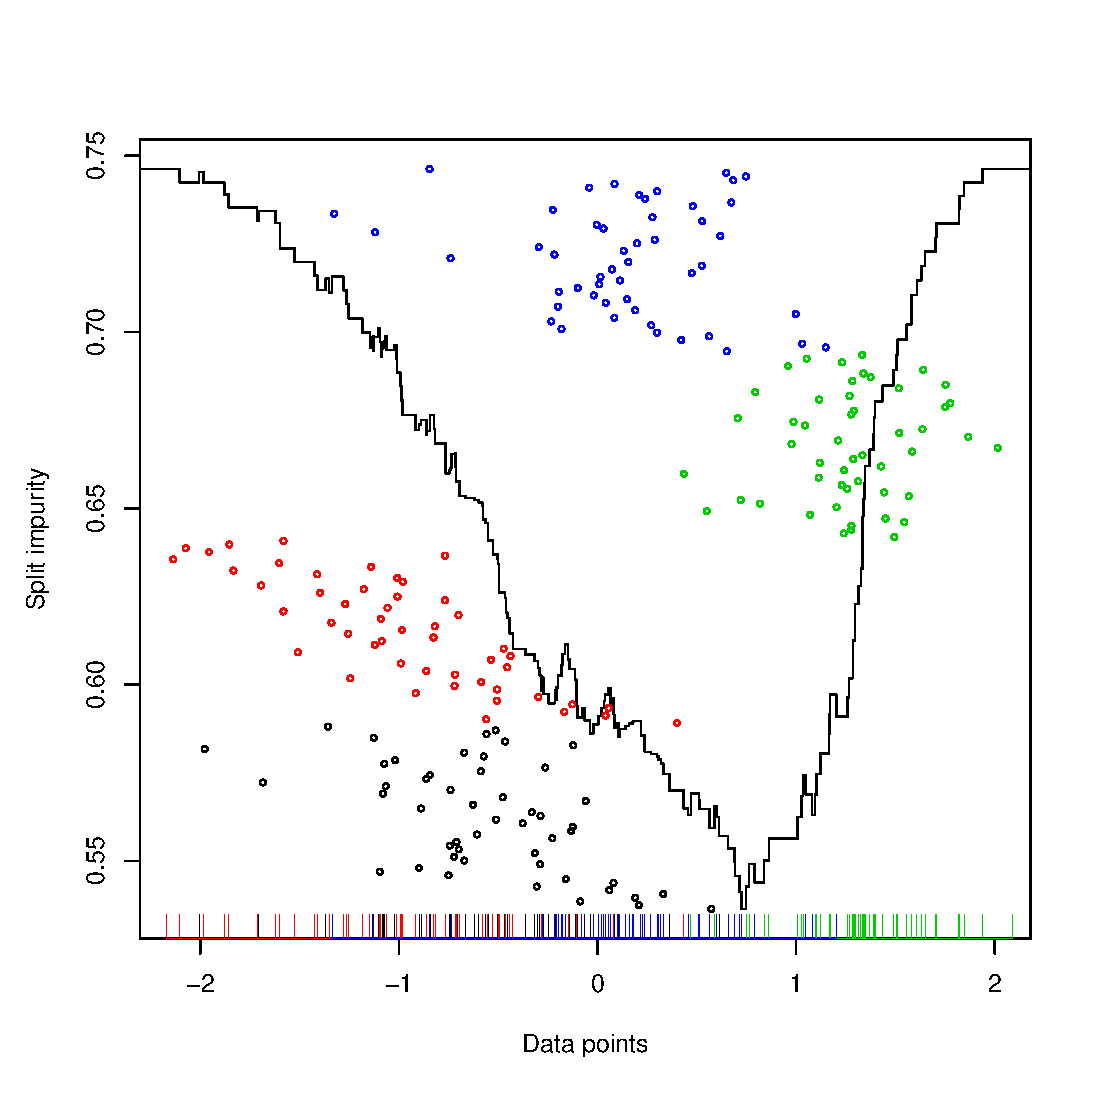
\includegraphics[width=.49\textwidth]{impurity_plot_1d_crabs_data_pc3.ps}
\caption{Plot showing smooth evolution of impurity measure over splits in the axis-parallel split dictionary}
\label{fig:impurity_plot_1d}
\end{figure}

For an arbitrary oblique split $\sum_{i=1}^q a_i X_i=c$, there is much greater freedom to produce similar splits. Increasing (or decreasing) any of the $q$ coefficients results in similar splits (failing to hold only in the unlikely event that many observations take the same value over \emph{all} $q$ continuous attributes). Though these $2^q$ similar splits need not produce unique outcomes, there are still anything between $2\leq m \leq 2^q$ similar outcomes to any given oblique split. Figure~\ref{fig:impurity_plot_2d} shows a typical evolution of the impurity measure when $q=2$.\\

\begin{figure}
\centering
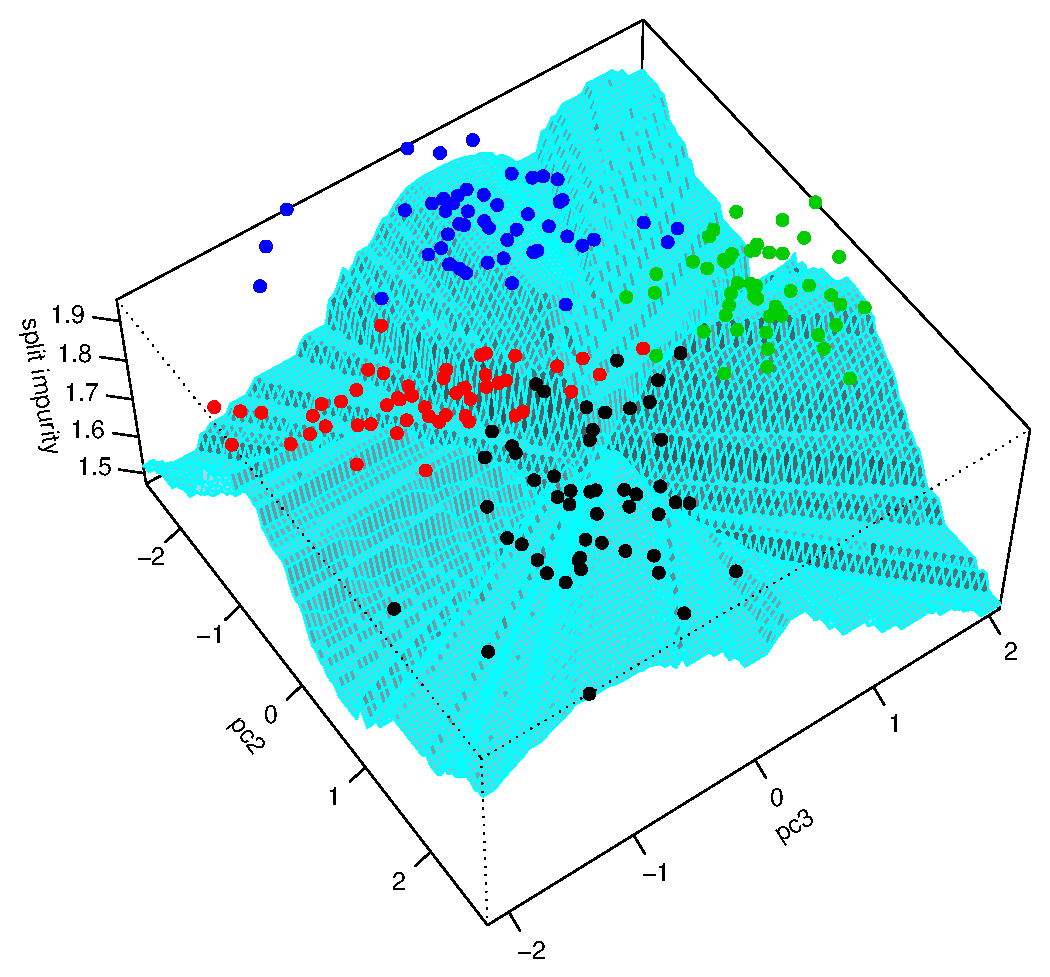
\includegraphics[width=.99\textwidth]{impurity_plot_2d_crabs_data_detail_100_bb.ps}
\caption{Plot showing smooth evolution of impurity surface over sampled splits from the oblique split dictionary}
\label{fig:impurity_plot_2d}
\end{figure}

As considering similar splits only yields marginal information about the impurity surface, it is desireable to avoid similar splits. As the impurity plots show, if observations of different classes lie in contiguous portions of the feature space, split impurity is low in areas \emph{between} these contiguous clusters of observations. For 1-dimensional plots in Figure~\ref{fig:impurity_plot_1d}, it is evident upon closer examination that kinks in the impurity measure occur where class clusters terminate. This phenomenon is particularly evident in Figure~\ref{fig:impurity_plot_2d}, where two valleys are formed which coincide in regions between class clusters. \\

By focusing on regions between class clusters, one can find splits with low impurity values. It is these regions that oblique splits identified in Section~\ref{IdealOutcomes} focus upon.
%Where contiguous structure is present in training data, the set of oblique splits mentioned in Section~\ref{IdealOutcomes} should naturally converge towards these points of interest due to the way in they are defined. 

%By only considering oblique splits that are derived from these ideal splits, not only do we have a much smaller set of splits to evaluate, each evaluated split should reveals a great deal about the impurity surface and such splits should be near to areas with relatively low values of impurity.\\

\begin{comment}
\section{Non-Contiguous and Non-Spherical Class Data}
\label{NonContiguousandNonSphericalClassData}
An obvious question that pops to mind when considering this heuristic argument is the following. When would the subset of oblique splits considered \emph{not} contain split with relatively low values of impurity? Where data is non-contiguous and where one wraps around the other!
\end{comment}


\chapter{Interpretable Oblique Trees}
\label{InterpretableObliqueTrees}
As interpretability is a key strength of classification trees, it is important to find ways of making oblique trees more interpretable. Apart from simply being small, guarding against unwarranted use of full oblique splits also helps trees to be more interpretable. Various approaches can be used to achieve this. They are categorised into two groups, 
\begin{description}
\item[During Tree Growth] methods applied during tree growth and 
\item[Post-Tree Growth] methods applied post-tree growth.
\end{description}
All methods use well-founded feature selection ideas introduced to trees by solving two-class classification problems during tree growth. Section~\ref{DuringTreeGrowth} covers methods applied during tree growth and Section~\ref{PostTreeGrowth} covers those applied post-tree growth.  

\section{During Tree Growth}
\label{DuringTreeGrowth}
Having seen how full oblique trees can be grown, it is easy to extend ideas in Chapter~\ref{InterpretableObliqueTrees} to grow concise oblique trees. When looking for the best split at each stage of tree growth, the set of full oblique splits can be substituted with a set of concise oblique splits. Instead of fitting logistic regression classifiers with all continuous attributes to two-class classification problems, feature selection techniques can be applied to remove attributes from the final model. This effectively produces concise oblique splits.\\

There are two established methods of finding succinct classifiers when fitting logistic regression classifiers, 
\begin{itemize}
\item Model Selection
\item Penalised Likelihood
\end{itemize}
Section~\ref{ModelSelection} expands on the use of model selection ideas and Section~\ref{PenalisedLikelihood} expands on penalised likelihood.\\

\noindent THE REST OF THIS CHAPTER MUST BE UPDATED\\
\noindent COMMENTS ARE WRITTEN IN BOLD

\subsection{Model Selection (1 MORE PAGE)}
\label{ModelSelection}
\noindent INTRODUCE AIC AND BIC\\
\noindent COMPARE AIC AND BIC, EXPLANATORY VS PREDICTIVE\\
\noindent TALK ABOUT R IMPLEMENTATION FOR MODEL SELECTION\\
\noindent GIVE EXAMPLES OF SUCH TREES\\

Akaike's \emph{An Information Criterion}~\cite{citeulike:849862} allows one to estimate the divergence between the log-likelihood of a probabilistic model trained on some dataset, to the log-likelihood of the same model on out-of-sample data (previously unobsersed data). A practical application of AIC involves augmenting the log-likelihood of a model by the infamous value $2q$ (where $q$ is the number of degrees of freedom of the model) which allows nested submodels to be compared on their (estimated) ability to accurately predict on out-of-sample data. The result of this procedure is that more succinct submodels may be preferred over the original model (which uses all $q$ attributes). In relation to logistic regression, attributes can be automatically removed from the model to produce concise oblique splits. \\

Schwarz's Information Criterion, more commonly known as the \emph{Bayesian Information Criterion}~\cite{citeulike:90008} provides a similarly practical result. Motivated through a bayesian framework, BIC penalises the log-likelihood of probabilistic models more severely than AIC and so for our purposes, produces oblique splits that are even more concise.\\

%COMPARE AIC AND BIC, BIC BEING EXPLANATORY MODEL (AND THUS MORE CONCISE SPLITS) AND AIC BEING PREDICTIVE (AND THUS LESS CONCISE)\\

\subsection{Penalised Likelihood (ANOTHER 3 PAGES)}
\label{PenalisedLikelihood}
\noindent EXPLAIN PENALISED LIKELIHOOD WORKS\\
%EXPLAIN HOW TO ACTUALLY USE IT TO GROW A TREE AS NEED TO SET LAMBDA FOR EACH NODE\\
\noindent SHOW HOW TO CAN BE USED WITH OBLIQUE TREES\\
\noindent TALK ABOUT R IMPLEMENTATION (USED GLMPATH) 
\noindent GIVE EXAMPLES OF SUCH TREES

\section{Post-Tree Growth}
\label{PostTreeGrowth}
Though methods presented in Section~\ref{DuringTreeGrowth} allow oblique trees with concise oblique splits to be grown, it is not easy to specify how concise such splits should be. Post-tree growth methods are better able to do this and allows the user to choose how interpretable the resulting tree should become. \\

\begin{comment}
Implicit in this approach is the assumption that unoptimised oblique trees are adept at capturing good tree structure albeit with more complicated splits at internal nodes than we would like. This assumption allows significant reduction in additional computation needed to find concise oblique trees. For both suggested approaches, we firstly grow an unoptimised oblique tree $T$ to some training data \emph{Tr}.\\
\end{comment}

Section~\ref{TreePruning} begins with the observation that traditional cost-complexity pruning methods can also be applied to the resulting oblique trees that are grown. %STILL NEED TO WRITE THIS

\subsection{Tree Pruning (ANOTHER 1/2 PAGE)}
\label{TreePruning}
\noindent COST-COMPLEXITY PRUNING ALSO WORKS WITH OBLIQUE TREES\\
\noindent TALK ABOUT R IMPLEMENTATION\\
\noindent GIVE AN EXAMPLES OF PRUNED OBLIQUE TREES 

By examining ideas behind cost-complexity pruning of axis-parallel trees, it is easy to see that such techniques are equally applicable to oblique trees. An large oblique tree can be pruned to reveal a family of rooted subtrees giving the user the ability to specify the size the of tree desired.\\


\subsection{\emph{Squeezing} Trees Using Shrinkage Methods}
\noindent NEED TO RETHINK THIS SECTION THROUGH \\
%\noindent TALK ABOUT LARS WHICH IS USED
%\noindent GIVE EXAMPLES OF THIS \\
%\noindent TALK ABOUT LARS WHICH IS USED

At any internal node $t$, we can fit a penalised logistic regression model to the data. By varying the value of the penalisation constant $\lambda_t$, we can \emph{squeeze} out unneccessary terms. Though different forms of penalisation ($L_1$, $L_2$, etc) affect the nature in which variables depart the model, this is immaterial at this stage of discussion. For each logistic regression model used at nodes $t$, it is important to note that $\lambda_t^{\mbox{max}}$ (the smallest value of $\lambda_t$ where the coefficients of the model are not affected by penalisation) varies significantly. I therefore feel that it is unwise to use a single numeric value of $\Lambda$ to simultaneuously penalise all logistic regression models in the oblique tree. Below are two better ways to holistically applying penalisation to logistic regression models in the tree,
\begin{description}
\item[Percentage-wise] Reducing a single term, the percentage $\Lambda_{\mbox{perc}}$, uniformly reduce the percentage of $\lambda_t^{\mbox{max}}$ used for the associated logistic regression models simultaneously
\item[Sum-wise] Reduce the single term $\Lambda_{\mbox{sum}}=\sum_{\mbox{nodes }t\mbox{ in }T}\lambda_t^{\mbox{max}}$, this forces all coefficients down to zero as $\Lambda_{\mbox{sum}}\rightarrow 0$
\end{description}
Though both approaches seem reasonable, sum-wise penalisation seems unneccessarily complicated to implement and so I prefer the percentage-wise approach. Having said this, my experience of using penalised logistic regression suggests that extracting the transition points of $\lambda_t$ where attributes leave the model is itself a difficult process. I have also noticed that the resulting logistic regression models do not remove terms with small coefficients as thoroughly as subset selection methods. This brings me to my preferred post-tree growth approach.\\

\subsection{Trimming Trees (ANOTHER 4 PAGES)}
\noindent IT IS POSSIBLE TO ADAPT COST-COMPLEXITY PRUNING TO PRUNE THE SPLITS OF A TREE RATHER THAN ITS NODES. DOING SO ALLOWS A GIVEN TREE TO BE \emph{TRIMMED} SO THAT MORE CONCISE OBLIQUE SPLITS ARE USED. THIS SECTION EXPANDS UPON THIS IDEA. UNFORTUNATELY, I HAVE NOT WRITTEN OUT THE CODE FOR IT YET AND SO IT CANNOT BE TESTED YET.\\
\noindent THIS SECTION EXPLAINS THIS IDEA, GIVING EXAMPLES AS WELL.

As with Breiman \emph{et al}, let $R(T)$ be a measure of the tree formed by adding contributions over its leaves and consider the penalised measure of fit $$R_\alpha(T)=R(T)+\alpha \mbox{comp}(T).$$ Here, we depart slightly from traditional theory by forming $\mbox{comp}(T)$ defined as follows, $$\mbox{comp}(T)=\sum_{B\mbox{: branches of }T}\frac{\mbox{\# attributes used over all internal nodes of }B}{\mbox{\# internal nodes of }B}.$$ Though this may appear complicated, it is instructive to note that $\mbox{comp}(T)$ collapses to the usual definition of $\mbox{size}(T)$ when $T$ is an axis-parallel tree. For oblique trees however, this measure further penalises trees that require more decision making to reach its leaves, it rightly skews our attention to trees that have simpler splits nearer the root node.\\

Traditional cost-complexity pruning seeks to find the smallest rooted subtree that minimises $R_\alpha(T)$ for some $\alpha$. We again depart slightly by seeking to minimise $R_\alpha(T)$ over a \emph{different} set of candidate trees, \emph{concise-trees}. For an oblique tree $T$, its family of \emph{concise-trees} has the same splitting structure in the sense that,
\begin{enumerate}
\item splits occur at the same internal nodes,
\item logistic regression models at internal nodes are based on the same partitioning of residual classes from the training set and
\item only a subset of the attributes used in the associated split of the original tree $T$ is permitted.
\end{enumerate}
Figure~\ref{fig:concisetreesandcomp} illustrates the concept of concise-trees and $\mbox{comp}()$ for individual branches more clearly. We wish to search over the set of concise-trees of $T$ to find the tree that minimises $R_\alpha(T)$ for some $\alpha$. \\

\begin{figure}
\centering
\includegraphics*[viewport=0 0 340 455]{figconcisetreesandcomp.eps}
\caption{Example of concise-trees and $\mbox{comp}(B)$ for a small oblique tree}
\label{fig:concisetreesandcomp}
\end{figure}

At this point, the elegant theory of cost-complexity pruning that allows efficient navigation over all rooted subtrees no longer holds for the more complicated family of concise-trees. Proposition 7.2 of Ripley's \emph{PPRN} allows for a fast and efficient search for $T(\alpha)$ (the smallest rooted subtree that minimises $R_\alpha$) for a particular $\alpha$. The simple structure of rooted subtrees is pivotal in allowing such a computational shortcut to exist, added complications of concise-trees lends no such luxury. Though it is theoretically possible to find the concise-tree with the smallest value of $R_\alpha$ (with the smallest value of $\mbox{comp}(T)$) by searching over the entire family, it would take too long in reality. The following greedy heuristic search however may prove promising.\\ 

We are firstly given some penalisation constant $\alpha$. For an internal node $t$ of an unoptimised oblique tree $T$, there are $n_t$ explanatory variables in the logistic regression model. Subset selection methods or shrinkage methods can reveal a new logistic regression model with $n_t-1$ terms which results in a new oblique split. The concise-tree $T_t^{\mbox{concise}}$ that replaces node $t$ with this new logistic regression model and leaves all other nodes untouched will have cost-complexity value $R_\alpha(T_t^{\mbox{concise}})$. Considering all such concise-trees by looking at all nodes $t$, we can greedily move to the concise-tree that gives the greatest reduction in $R_\alpha$. When $R_\alpha$ reaches a minimum, we accept this concise-tree $T_\alpha^{\mbox{heur}}$ as our approximation to $T_\alpha$, the best concise-tree.\\

Proposition 7.3 of Ripley's \emph{PPRN} allows efficient traversal of all interesting values of $\alpha$. Again, this shortcut is not accessible for our more complex family of concise-trees. A brute force approach to find $T_\alpha^{\mbox{heur}}$ over a mesh of values of $\alpha$ seems feasible, we can stop searching when $T_\alpha^{\mbox{heur}}$ becomes the trivial tree. \\

This approach allows a family of concise-trees with small value of $R_\alpha$ to be extracted from an unoptimised oblique tree from which the best generalising concise-tree can be chosen as usual.
\chapter{Additional Points}
\label{AdditionalPoints}
There are several issues related to the use of this method on real datasets I want to bring forth in this chapter. %This section will be divided into weaknesses and strengths of the method.\\

\section{Weakness}
\label{Weakness}
\subsection{Poor Oblique Splits (ANOTHER 5 PAGES)}
\label{PoorObliqueSplits}
I believe that are times when the approach taken in Section~\ref{ObliqueSplitsviaProbabilisticModels} may fail to provide good oblique splits. Situations include the case where class data is non-contiguous, and non-spherical. If this were the case, oblique splits found in this way are not attracted to areas of low impurity values. This needs to be investigated further.\\

\subsection{Complexity Analysis (ANOTHER 3 PAGES)}
\label{ComplexityAnalysis}
A investigation on the computational complexity of techniques mentioned in this thesis needs to be done. This should highlight situations where this approach to growing oblique trees does not perform well. A definite area of weakness includes the case where there are a great number of classes in the classification dataset. It may also perform poorly in the situation where there are many continuous attributes also. May also include comparison with existing methods of oblique tree growth.\\

\begin{comment}
\section{Strengths}
\label{Strengths}
\subsection{Rotational Invariance (ANOTHER 2 PAGES)}
\label{Rotational Invariance}
By allowing oblique splits, oblique trees are invariant to rotations in the dataset unlike axis-parallel trees. It would be useful to demonstrate this by rotating a dataset and growing axis-parallel and oblique trees on them to show this invariance.\\
\end{comment}

\chapter{Concluding Remarks (ANOTHER 2 PAGES)}
\label{ConcludingRemarks}
Final remarks. This will contain my thoughts of the implications of this work. Mention R package will be provided (not that it can be made faster). Touch upon addition research areas.\\

\begin{itemize}
\item Using ideal splits as starting points for hill-climbing methods
\item Extending idea to regression trees, using clustering methods
\item Random forests idea over classes to speed up tree growth for large problems
\item Provide an implementation in C to speed up existing R work
\end{itemize}
\singlespacing

\pagestyle{plain}

\bibliography{bib}
\bibliographystyle{plain}

\end{document}
